\documentclass[10pt,a4paper]{article}
\usepackage[utf8]{inputenc}
\usepackage{amsmath}
\usepackage{amsfonts}
\usepackage{amssymb}
\usepackage{amsthm}



\usepackage{float}
\usepackage{subfigure}
\usepackage{framed}
\usepackage{xcolor}

\usepackage{hyperref}
\hypersetup{
  colorlinks   = true, %Colours links instead of ugly boxes
  urlcolor     = red, %Colour for external hyperlinks
  linkcolor    = black, %Colour of internal links
  citecolor   = blue %Colour of citations
}

\usepackage{graphicx}
\graphicspath{{images2/}}

\definecolor{shadecolor}{gray}{0.9}

% Operators
\DeclareMathOperator*{\argmax}{arg\,max}
\DeclareMathOperator*{\argmin}{arg\,min}
\DeclareMathOperator*{\argminA}{arg\,min} % Jan Hlavacek

% Environments theorems
\newtheorem{questions}{Question}
\newenvironment{question}
   {\begin{shaded}\begin{questions}}
   {\end{questions}\end{shaded}}

\author{Ram\'on Mart\'inez}
\title{BCPNN and Sequence Learning}

% Paragraph parameters
\setlength{\parskip}{1em}

\begin{document}
\maketitle

\section{Introduction}

Generalities about the neccessity of including sequence processing capabilities on our models.

Why the problem of sequences in attractor neural networks (cite work of Amari, Sampolinsky).

More modern attemps like Verduzco, Fiete, and point out their limitations as models. 

Describe what exactly you are going to do: introduce the model, explain the architecture, show that it possess wide dynamical range, then show that it can learn sequences and characterize this process, describe its how sensitivity it is to noise, show that it can learn non-ortoghonal representation. 

\section{Results}

Description of the model. 

We present a firing rate motel (of the cortex?) where the synaptic input evolves according the equation \ref{eq:current} and binary activity indicator functions $\mathbf{o}$ that responds istantenously to synaptic input y through a softmax function as indicated in equation \ref{eq:non-linearity}. Describe winner take all dynamics. Furthermore the synaptic inputs are subjected to an adaptation current (synaptic depression? spike-frequency adaptation?). 

\begin{align}
\tau_s \dfrac{ds_i}{dt} &= \beta_i + \sum_{j} w_{ij} o_j  - g_a a_i - s_i  + \xi(t) \label{eq:current} \\ 
\tau_a \dfrac{da_i}{dt} &= o_i - a_i \label{eq:adaptation} \\
o_i &=   \begin{cases}
       1,&  s_i = \underset{hypercolumn}{\max}(\mathbf{s}),\\
       0 ,& \text{otherwise}
    \end{cases} \label{eq:non-linearity}
\end{align}


\begin{figure}[H]
\centering
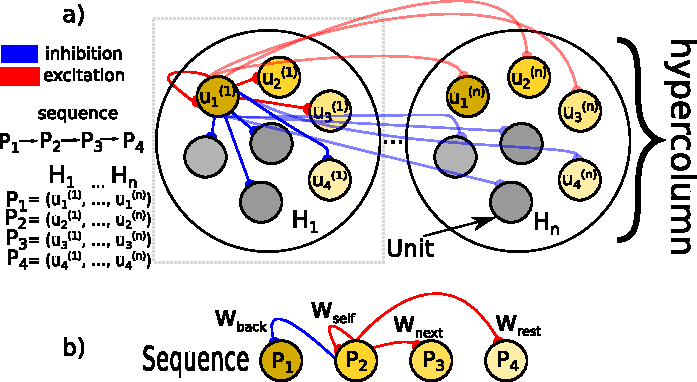
\includegraphics[scale=1.0]{diagram.pdf}
\caption{Schematic of the network structure. Units are organized into hypercolumns $H_1$, $\ldots$, $H_n$. At each point in time only one unit is active in each of the hypercolumns (small black circles). Patterns are defined as set of activated units across the hypercolumns. Pattern A, for example is the activation of unit 1 all the hypercolumns and can be represented by $A=(1, \ldots, 1)$. We depict stereotypical network connectivity by showing all the units that emanate from unit 1. The unit connects in excitatory fashion to the proximate units on the sequence (connections from 1 to 2 and 3) but it connects in an inhibitory fashion to both the units that are farther ahead on the sequence (1 to 4) and not in the sequence at all (1 to gray units). In the bottom In the first section of this work we will be working with only one hypercolumn, that is, we will be only using the connectivity inside the dashed gray box to the left of the diagram.}
\label{fig:networks_scheme}
\end{figure}




\subsection{The system can recall sequences}


When the unit is activated by the cue the adaptation current from equations \ref{eq:current} and \ref{eq:current} immediately starts eroding the pattern. As soon as the the total current (self-excitation minus adaptation) becomes weaker than feed-forward current to the next element the non-linearity in equation \ref{eq:non-linearity} kicks-in and suppresses the unit activated the next, we say that a transition has occurred and we call the time it took between those two events the persistence time of the attractor $T_{persistence}$. The next unit will be subjected to the same process of erosion by the adaptation current and in consequence the sequence will propagate in the network. \ref{fig:recall}. 

\begin{figure}[H]
\centering
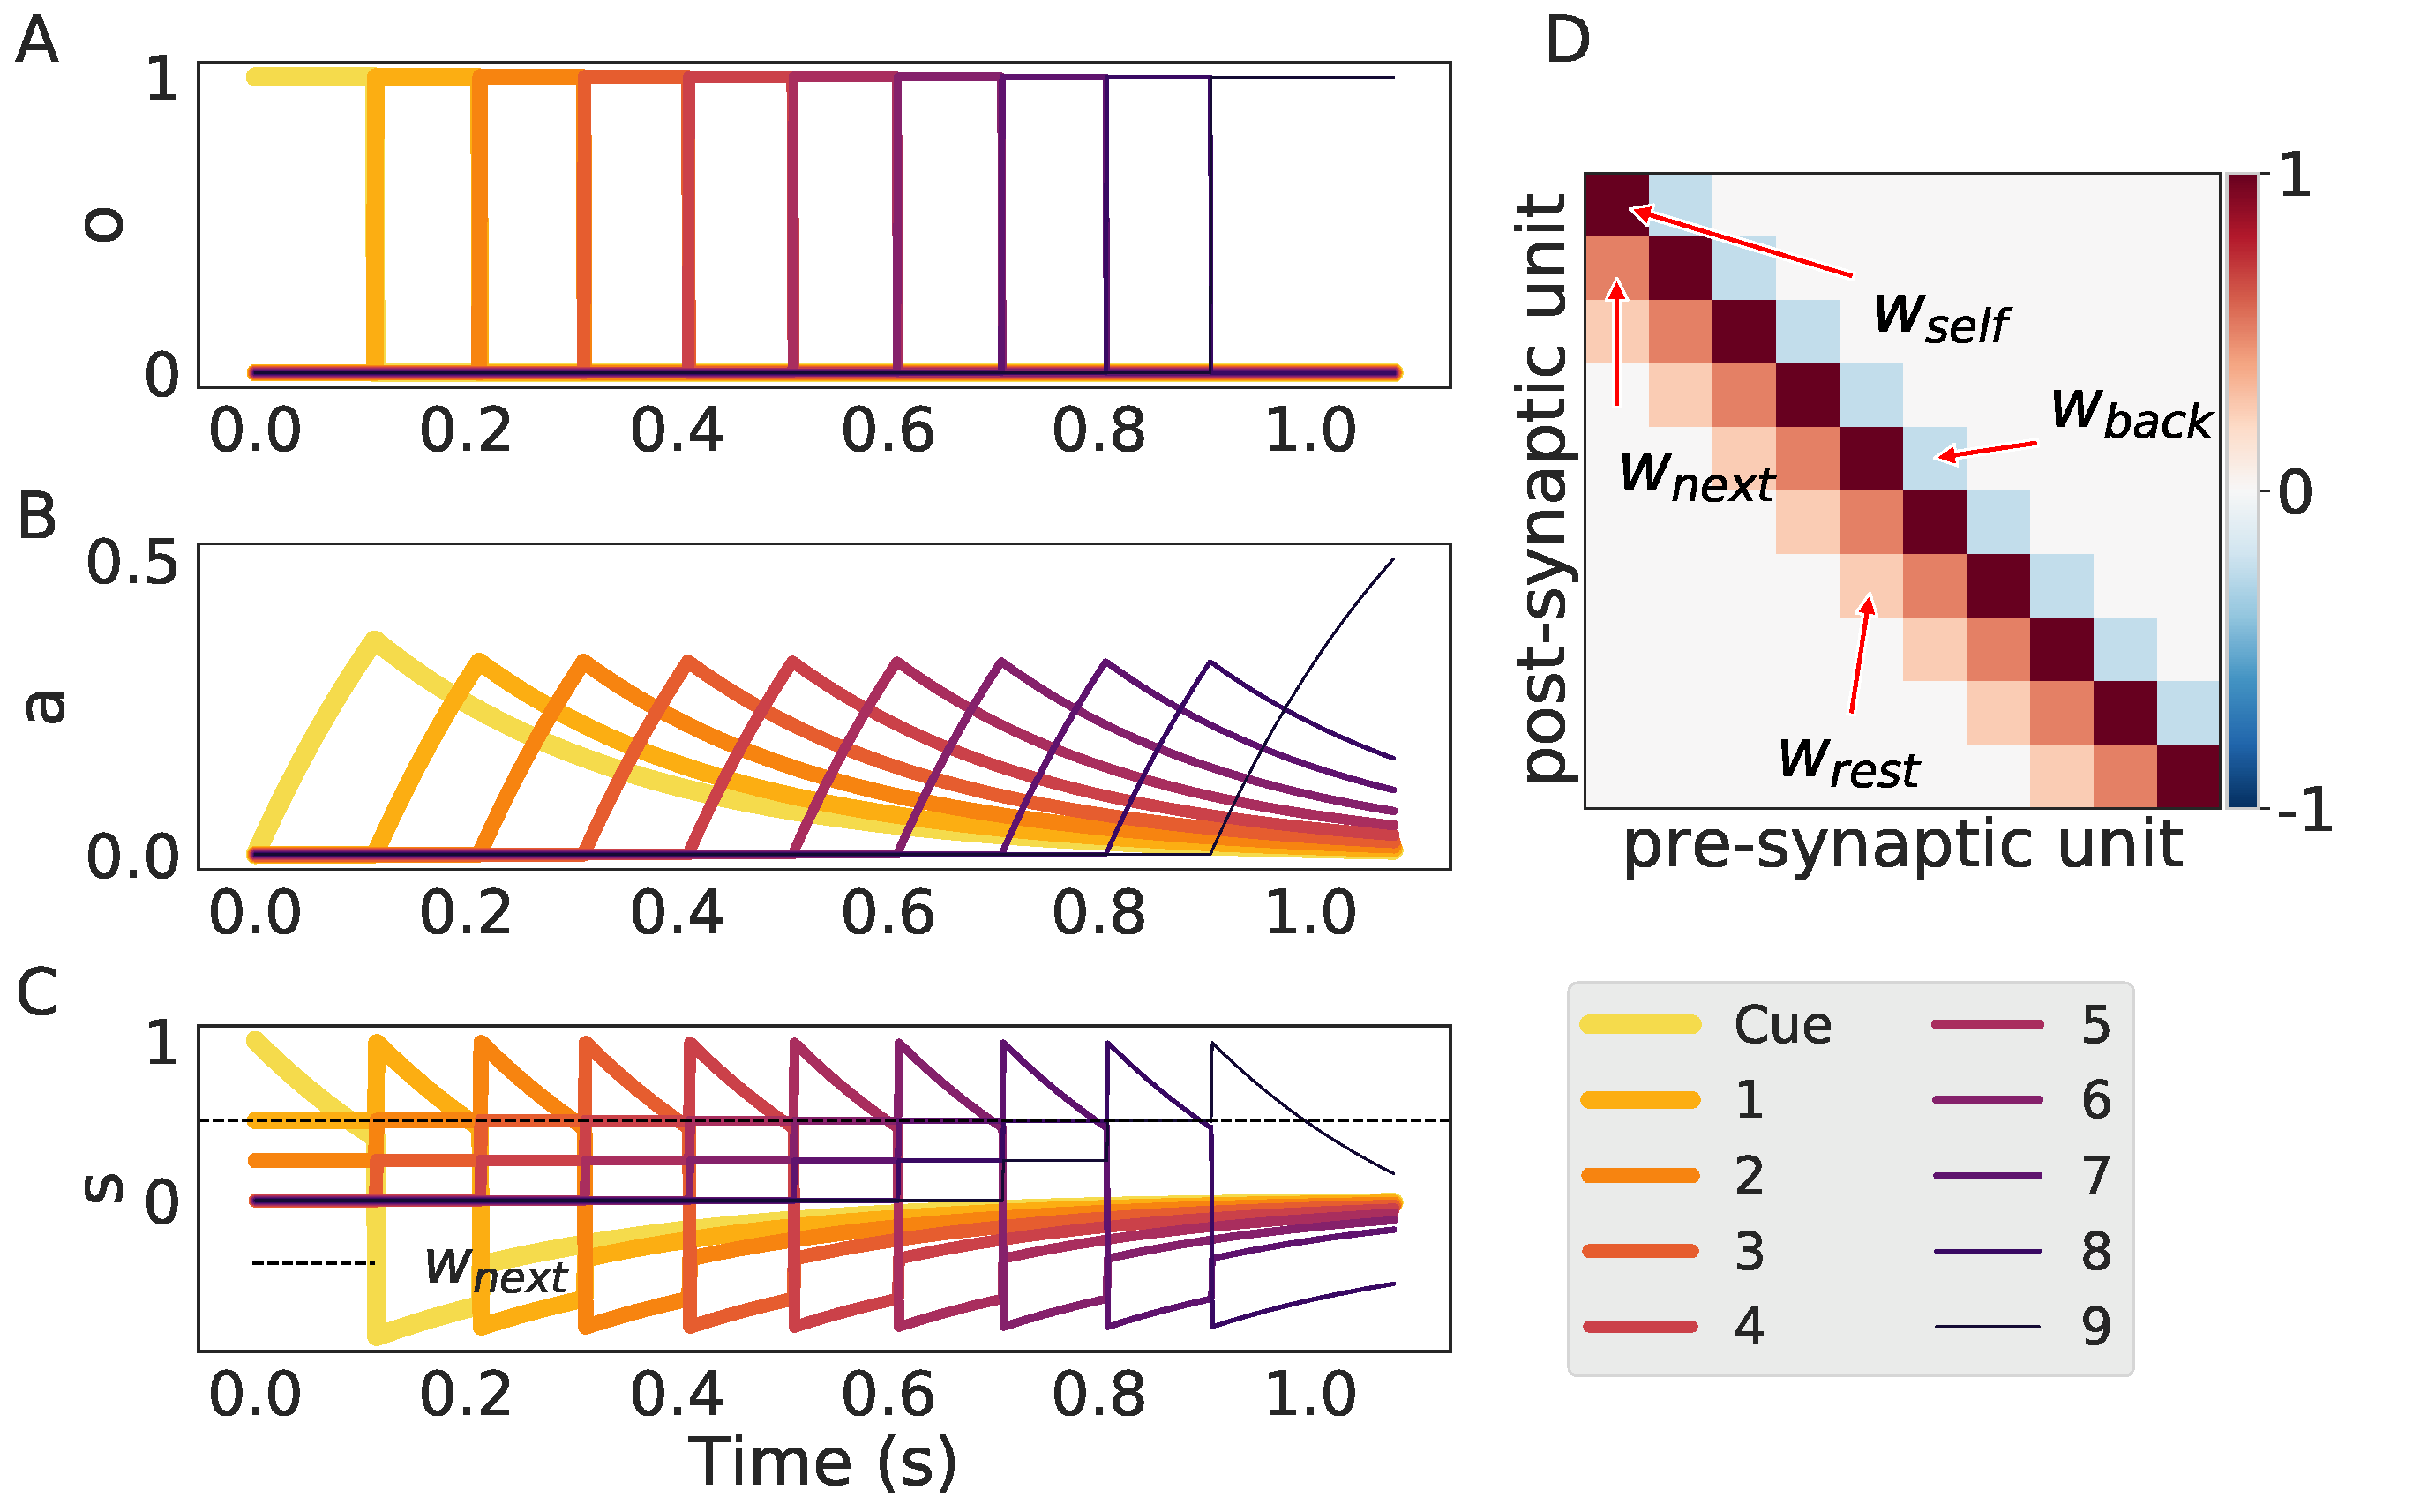
\includegraphics[scale=0.25]{simple_bcpnn_recall.pdf}
\caption{An instance of recall in the neural network. a) Unit activity starting with the cue. b) the time course of the adaptation current for each unit. c) total current is equal to self-excitatory current minus the adaptation current, note that this quantity crossing the value of $w_{next}$ (depicted here with a dotted line) marks the transition point from one unit to the next. d) The connectivity matrix where we have included pointers to the most important quantities $w_{self}$ for the self-excitatory weight, $w_{next}$ for the inhibitory connection to the next element, $w_{rest}$ for the biggest connection in the column after $w_{next}$ and finally $w_{back}$ for the connection to the last unit that was active on the sequence.}
\label{fig:recall}
\end{figure}



\subsection{Persistent time}

\begin{align}
T_{persistence} = \tau_a \log \left(\frac{1}{1 - B} \right) + \tau_a \log \left( \frac{                                                                                                                                                                                     1}{1 - \frac{\tau_s}{\tau_a}} \right)  \\ \label{eq:persistent_times}
B = \frac{w_{self} - w_{next} + \beta_{self} - \beta_{next}}{g_a} = \frac{\Delta w_{next} + \Delta \beta_{next}}{g_a}
\end{align}


From equation \ref{eq:persistent_times} we infer that we need $0 < B < 1$ for the transition to occur. As illustrated illustrate in \ref{fig:per_time}a) $T_{persistence}$ is small for $B \sim 0$ and diverges to infinity as $B \sim 1$. Which allow us to interpret B as a the


\begin{figure}[H]
\centering
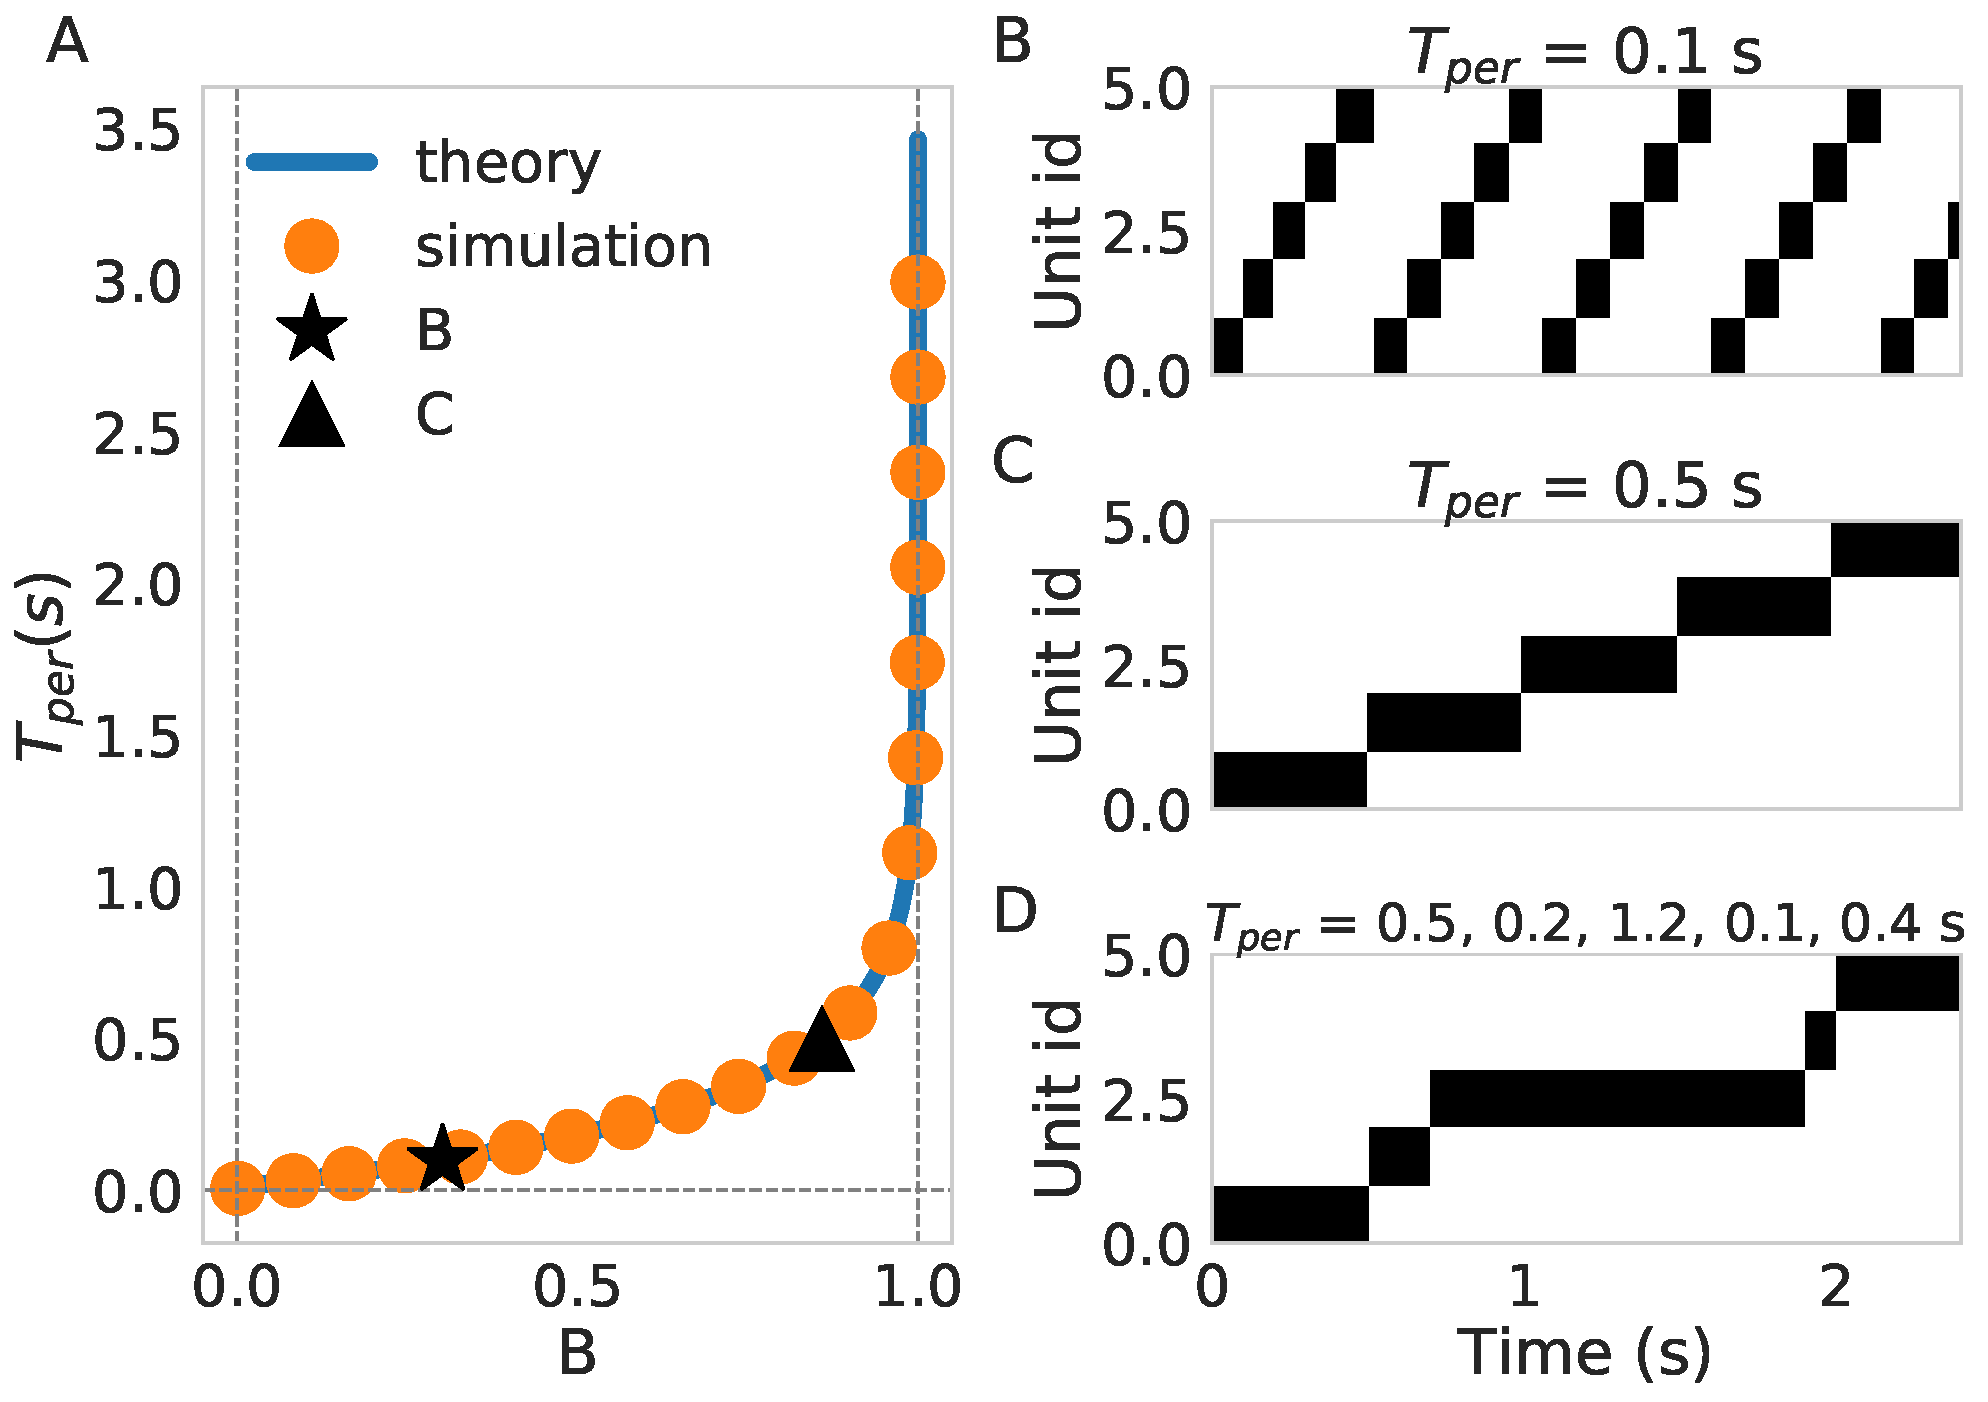
\includegraphics[scale=0.30]{persistent_times.pdf}
\caption{A characterization of persistent times. a) we show here that by controlling the parameter B between 0 and 1 we can control the persistent time of the system. To the right we show two examples of encoding first on b) there is an example of a sequence with small persistent time and  in c) another example with longer persistent time.}
\label{fig:per_time}
\end{figure}

\subsection{Learning}

\begin{align}
\tau_{z_{post}} \dfrac{dz_i}{dt} &= o_i - z_i 
& \tau_{z_{pre}} \dfrac{d z_j}{dt} &= o_j - z_j \label{eq:z_traces} \\
t \dfrac{dp_i}{dt} &= z_i - p_i  
\qquad \quad t\dfrac{dp_{ij}}{dt} = z_i z_j - p_{ij}
&t\dfrac{dp_j}{dt} &= z_j - p_j    \label{eq:p_traces} \\
w_{ij} &= \log \left(\frac{p_{ij}}{p_i p_j} \right) & \beta_i &= \log(p_i) \label{eq:bcpnn} 
\end{align}

%\begin{align}
%\tau_{z_{post}} \dfrac{d\underset{post}{z_i}}{dt} &= o_i - \underset{post}{z_i} 
%& \tau_{z_{pre}} \dfrac{d\underset{pre}{z_i}}{dt} &= o_i - \underset{pre}{z_i} \label{eq:z_traces} \\
%t \dfrac{dp_i}{dt} &= \underset{pre}{z_i} - p_i  
%\qquad \quad t\dfrac{dp_{ij}}{dt} = z_i z_j - p_{ij}
%&t\dfrac{dp_i}{dt} &= \underset{pre}{z_i} - p_i    \label{eq:p_traces} \\
%w_{ij} &= \log(\frac{p_{ij}}{\underset{pre}{p_i} \quad\underset{post}{ p_j}}) & \beta_i &= \log(p_i) \label{eq:bcpnn} 
%\end{align}

\begin{figure}[H]
\centering
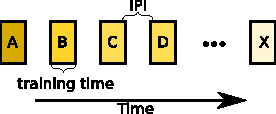
\includegraphics[scale=1.40]{protocol.pdf}
\caption{The training protocol. We show here the basic scheme of the training protocol used in the system. The training protocol can be characterized first by the training time of each unit, that is, how long is the system exposed (units are clamped) to the pattern and second by the inter pulse interval (IPI) of each pair of units which is the dead time in between their activation. Note that while this need not to be equal for each pattern we will characterize in the following an homogeneous training protocol.}
\label{fig:training_protocol}
\end{figure}


\begin{figure}[H]
\centering
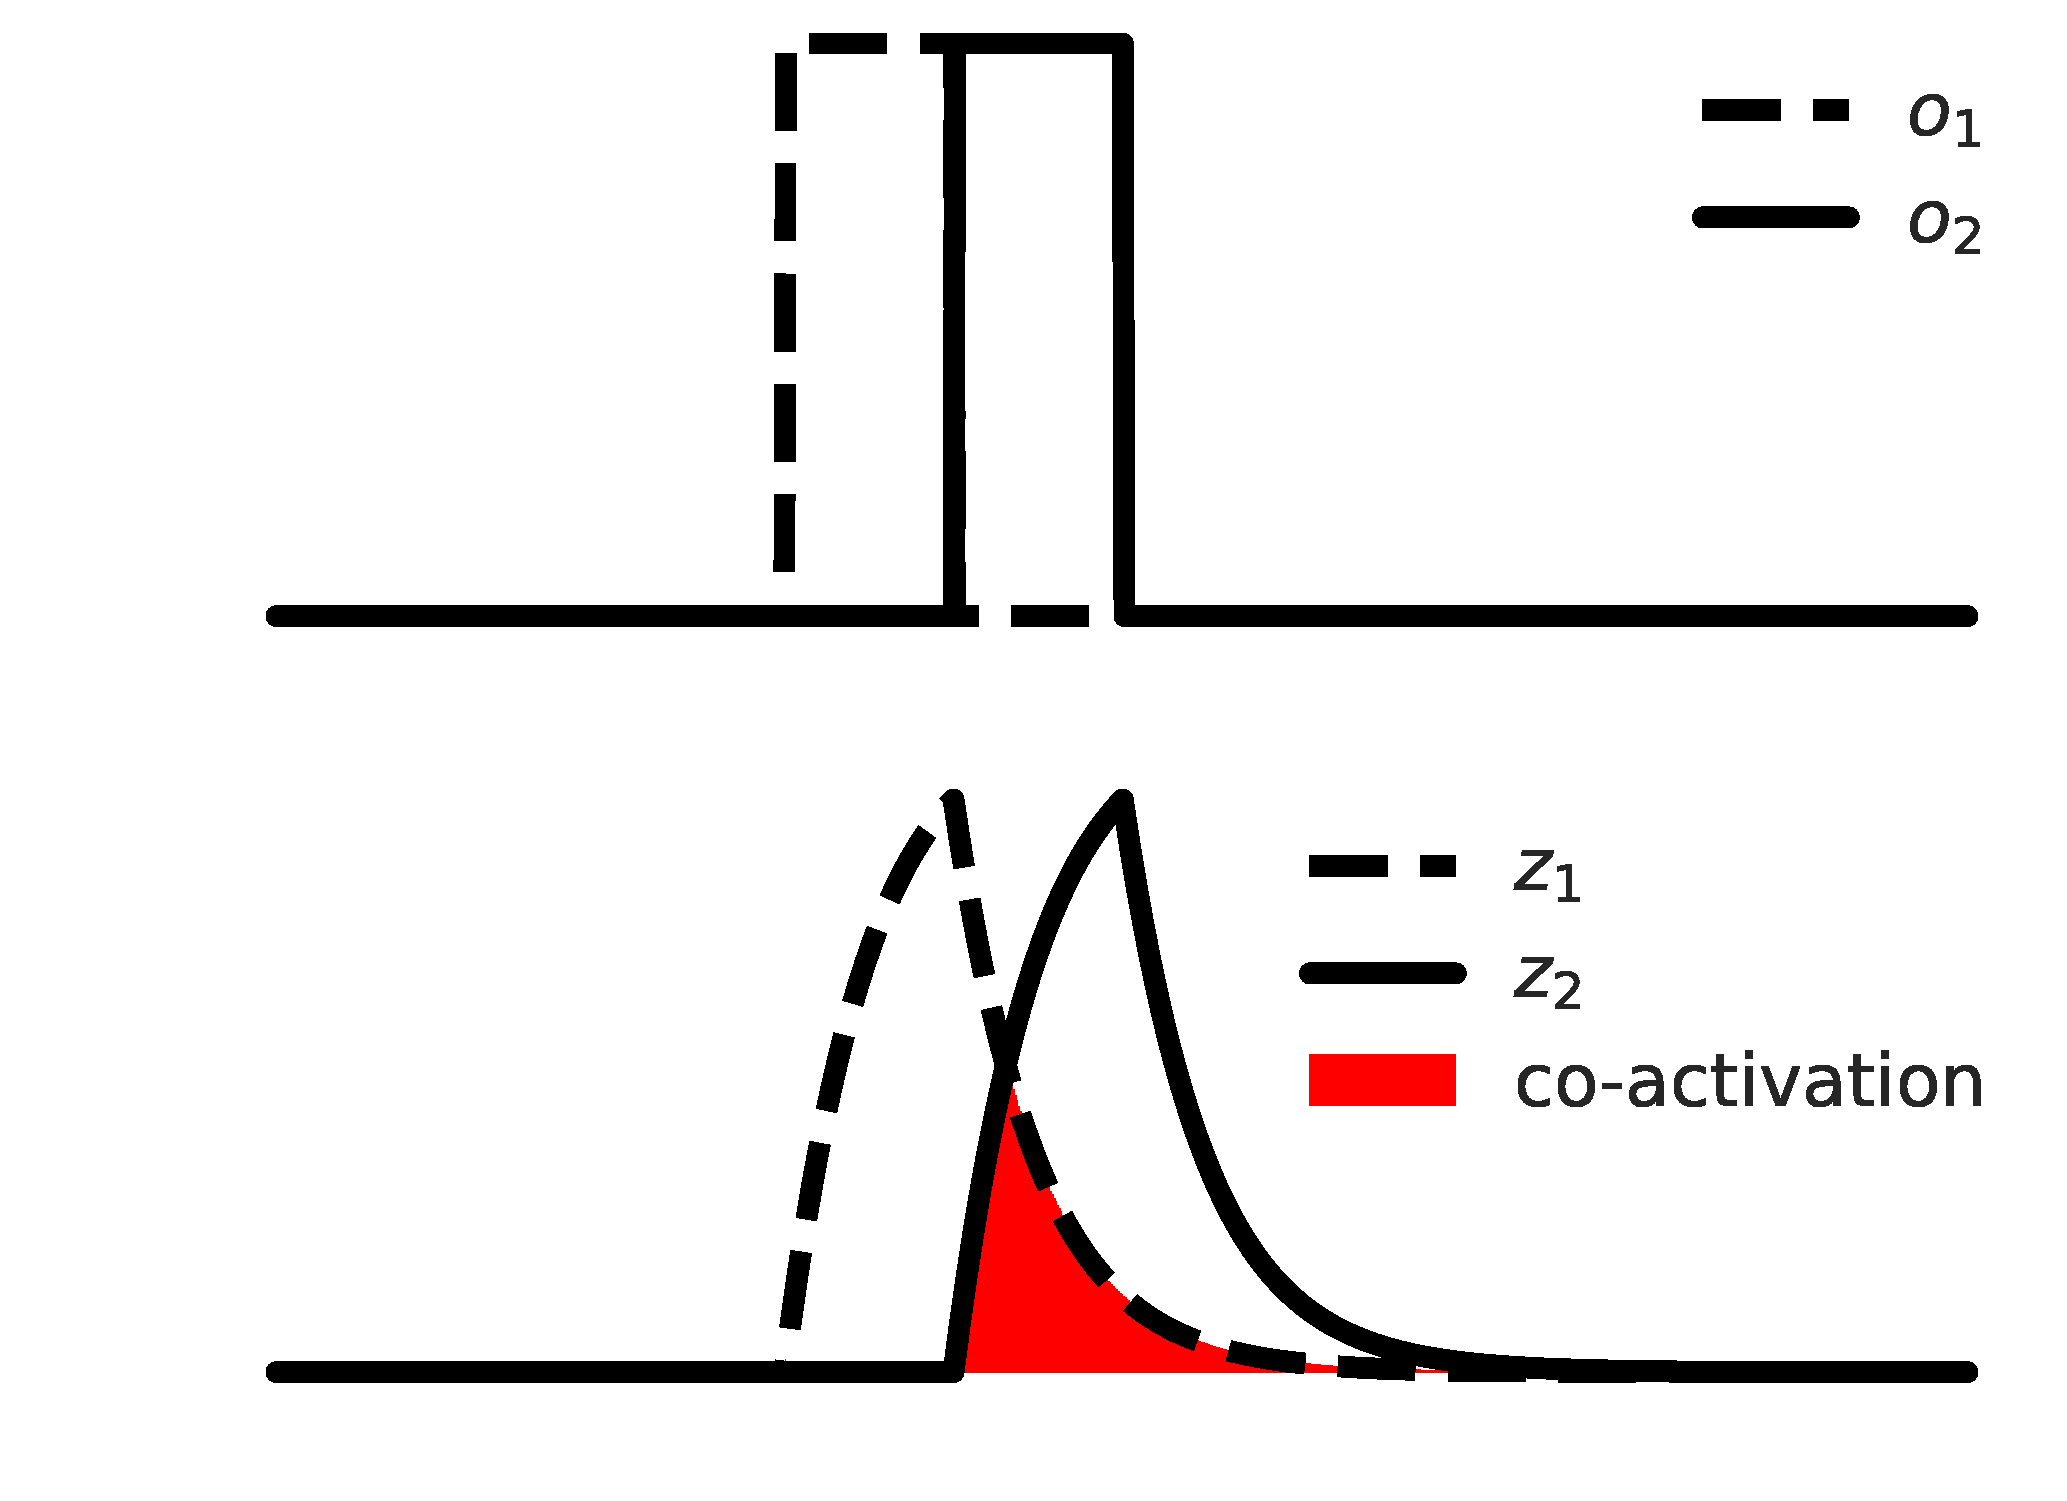
\includegraphics[scale=0.30]{traces_example.pdf}
\caption{Learning by traces. The system weights the intersection of two traces (co-activation) against the base activation rate of each unit to determine the magnitude of the weight between two units. }
\label{fig:traces_example}
\end{figure}

\begin{figure}[H]
\centering
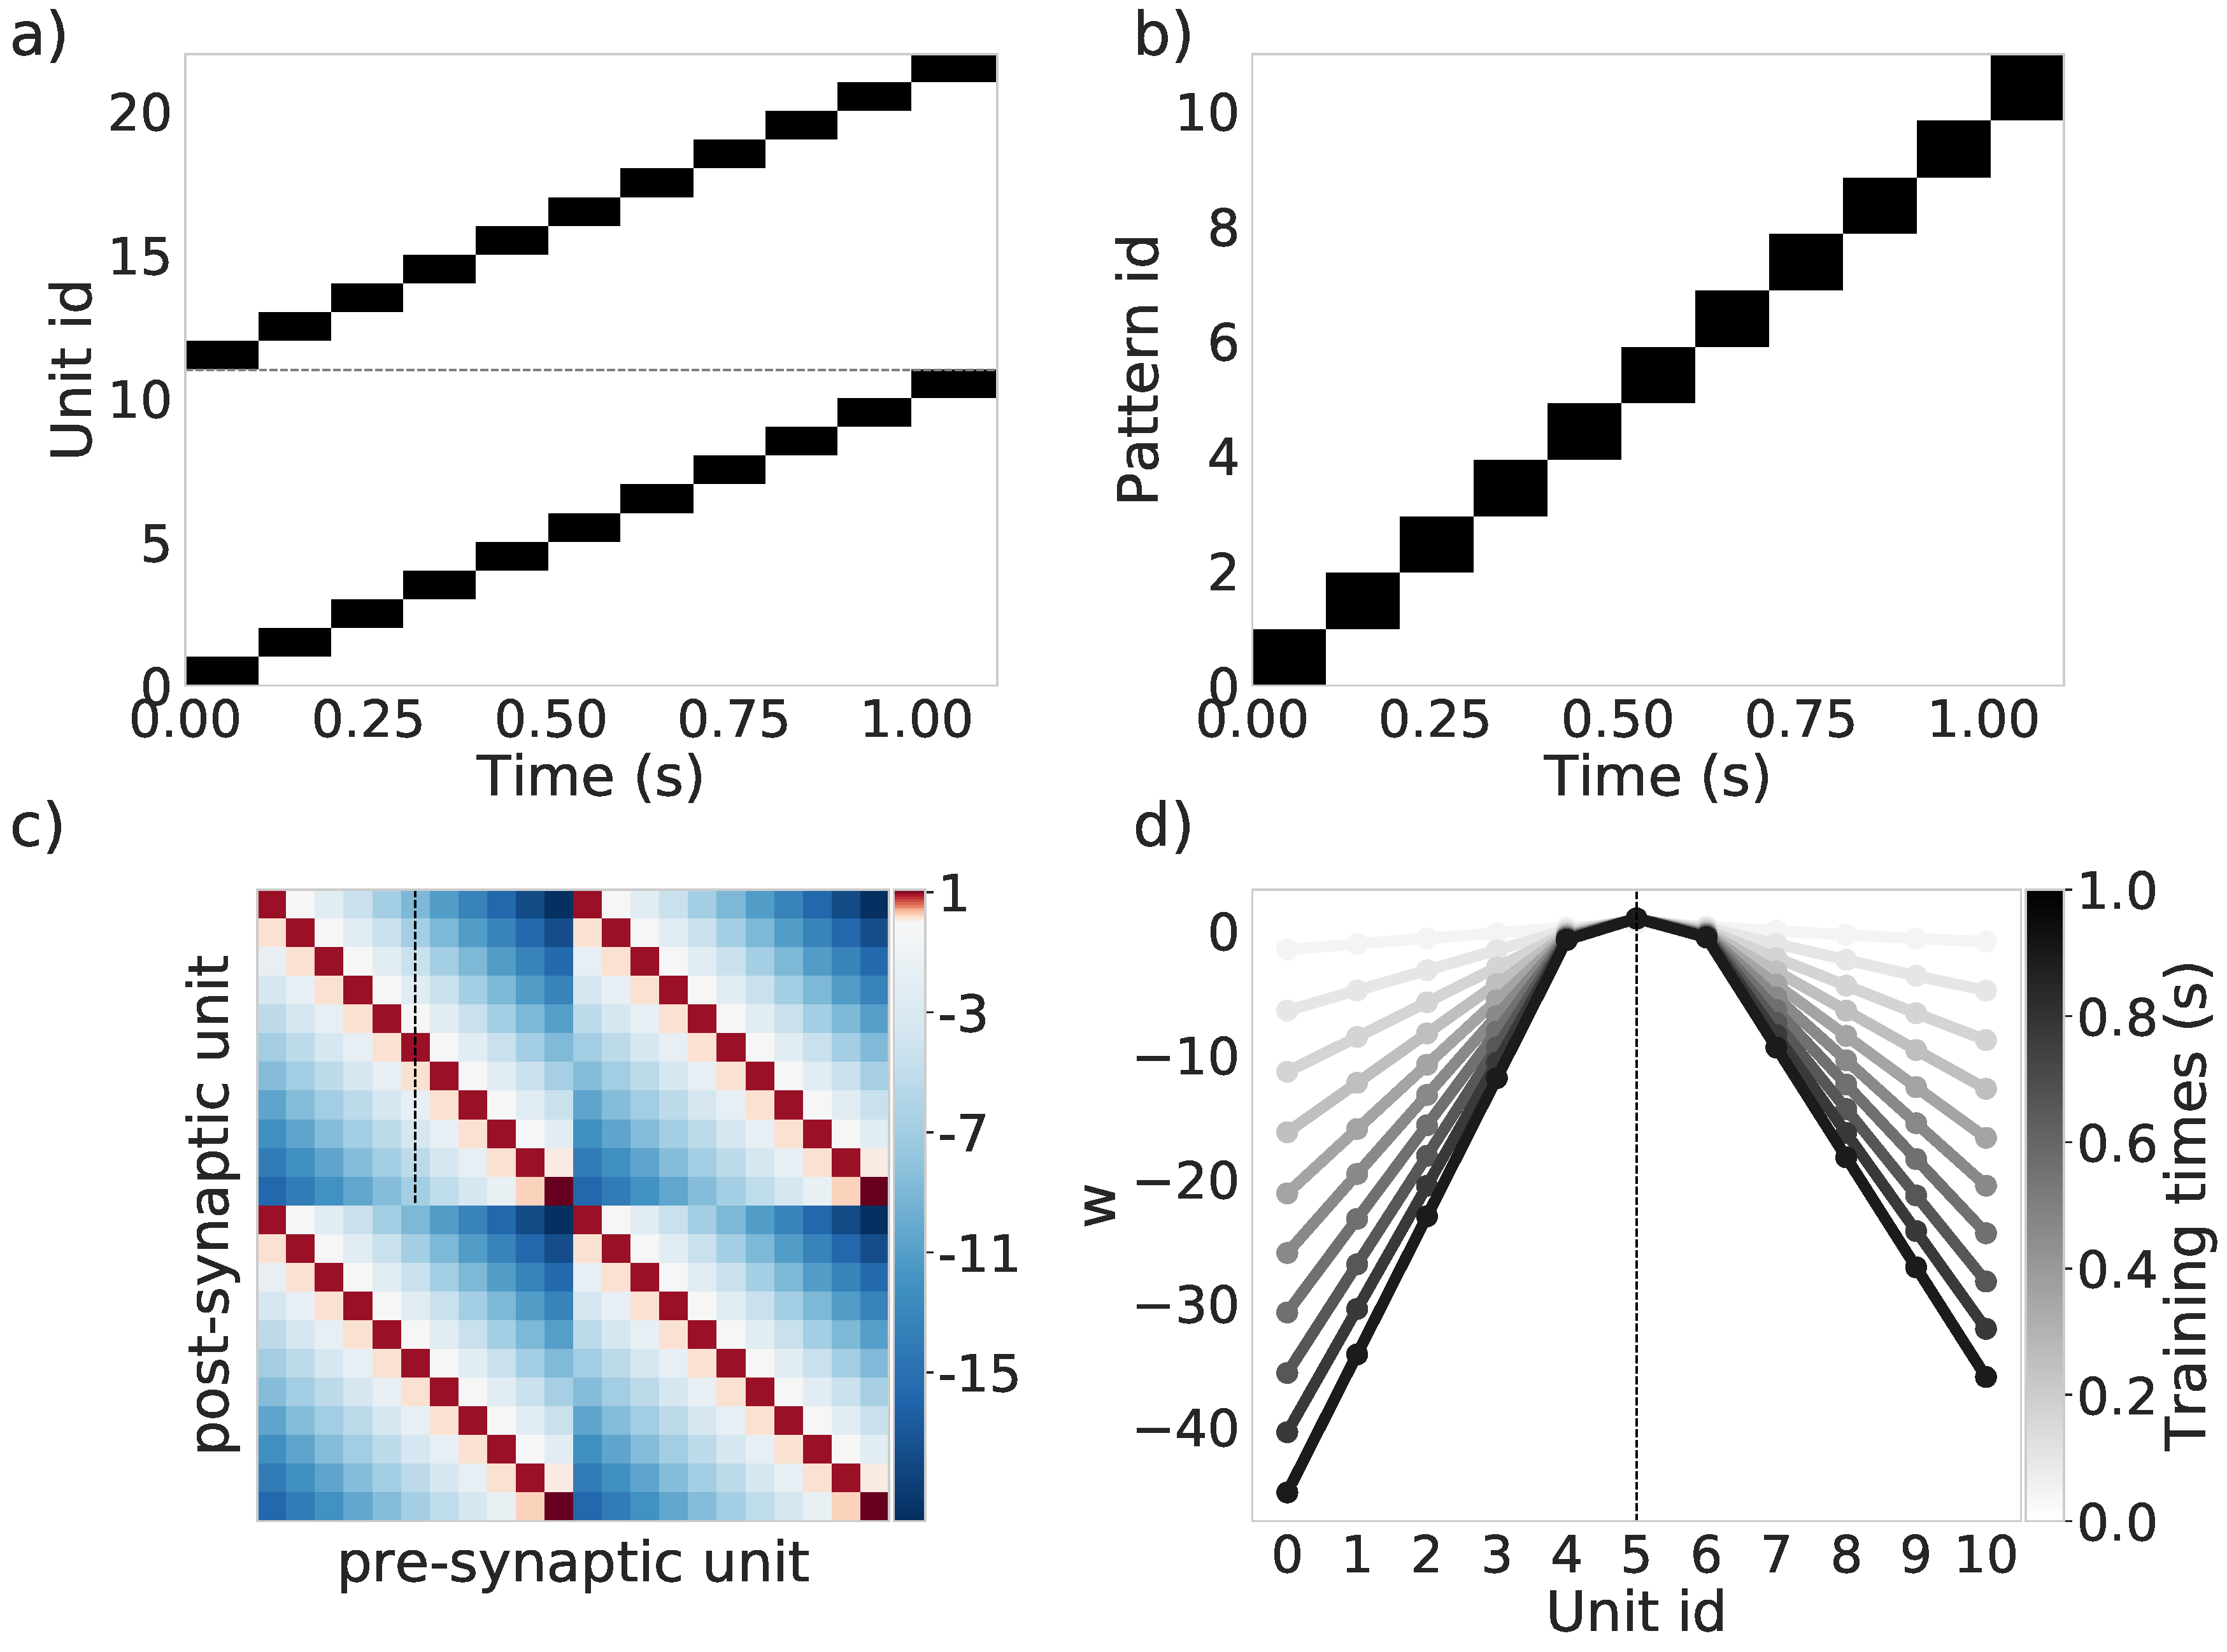
\includegraphics[scale=0.20]{recall_example.pdf}
\caption{An example of recall with 10 minicolumns and 2 hypercolumns, $\tau_{z_{pre}} = \tau_{z_{post}}=25 \, ms$, training times $=100 \, ms$ and $IPI = \, 0 $. We show in a) how the recall phase in a system with learned connectivity looks like. The division by hypercolumns is marked with a horizontal dashed line b) We show how close (1 - cosine distance) the instant activity of the network is to the stored pattern at every point in time. c) The connectivity matrix for this particular example, note the the organization is an outcome of the modularity of connectivity. Finally to illustrate the dependency of connectivity on the training protocol we show the profile of connections of the dashed line on d) for a variety of training times (ten examples from from 100 ms to 1s). Darker lines represent longer training times.}
\label{fig:recall_example}
\end{figure}


\begin{figure}[H]
\centering
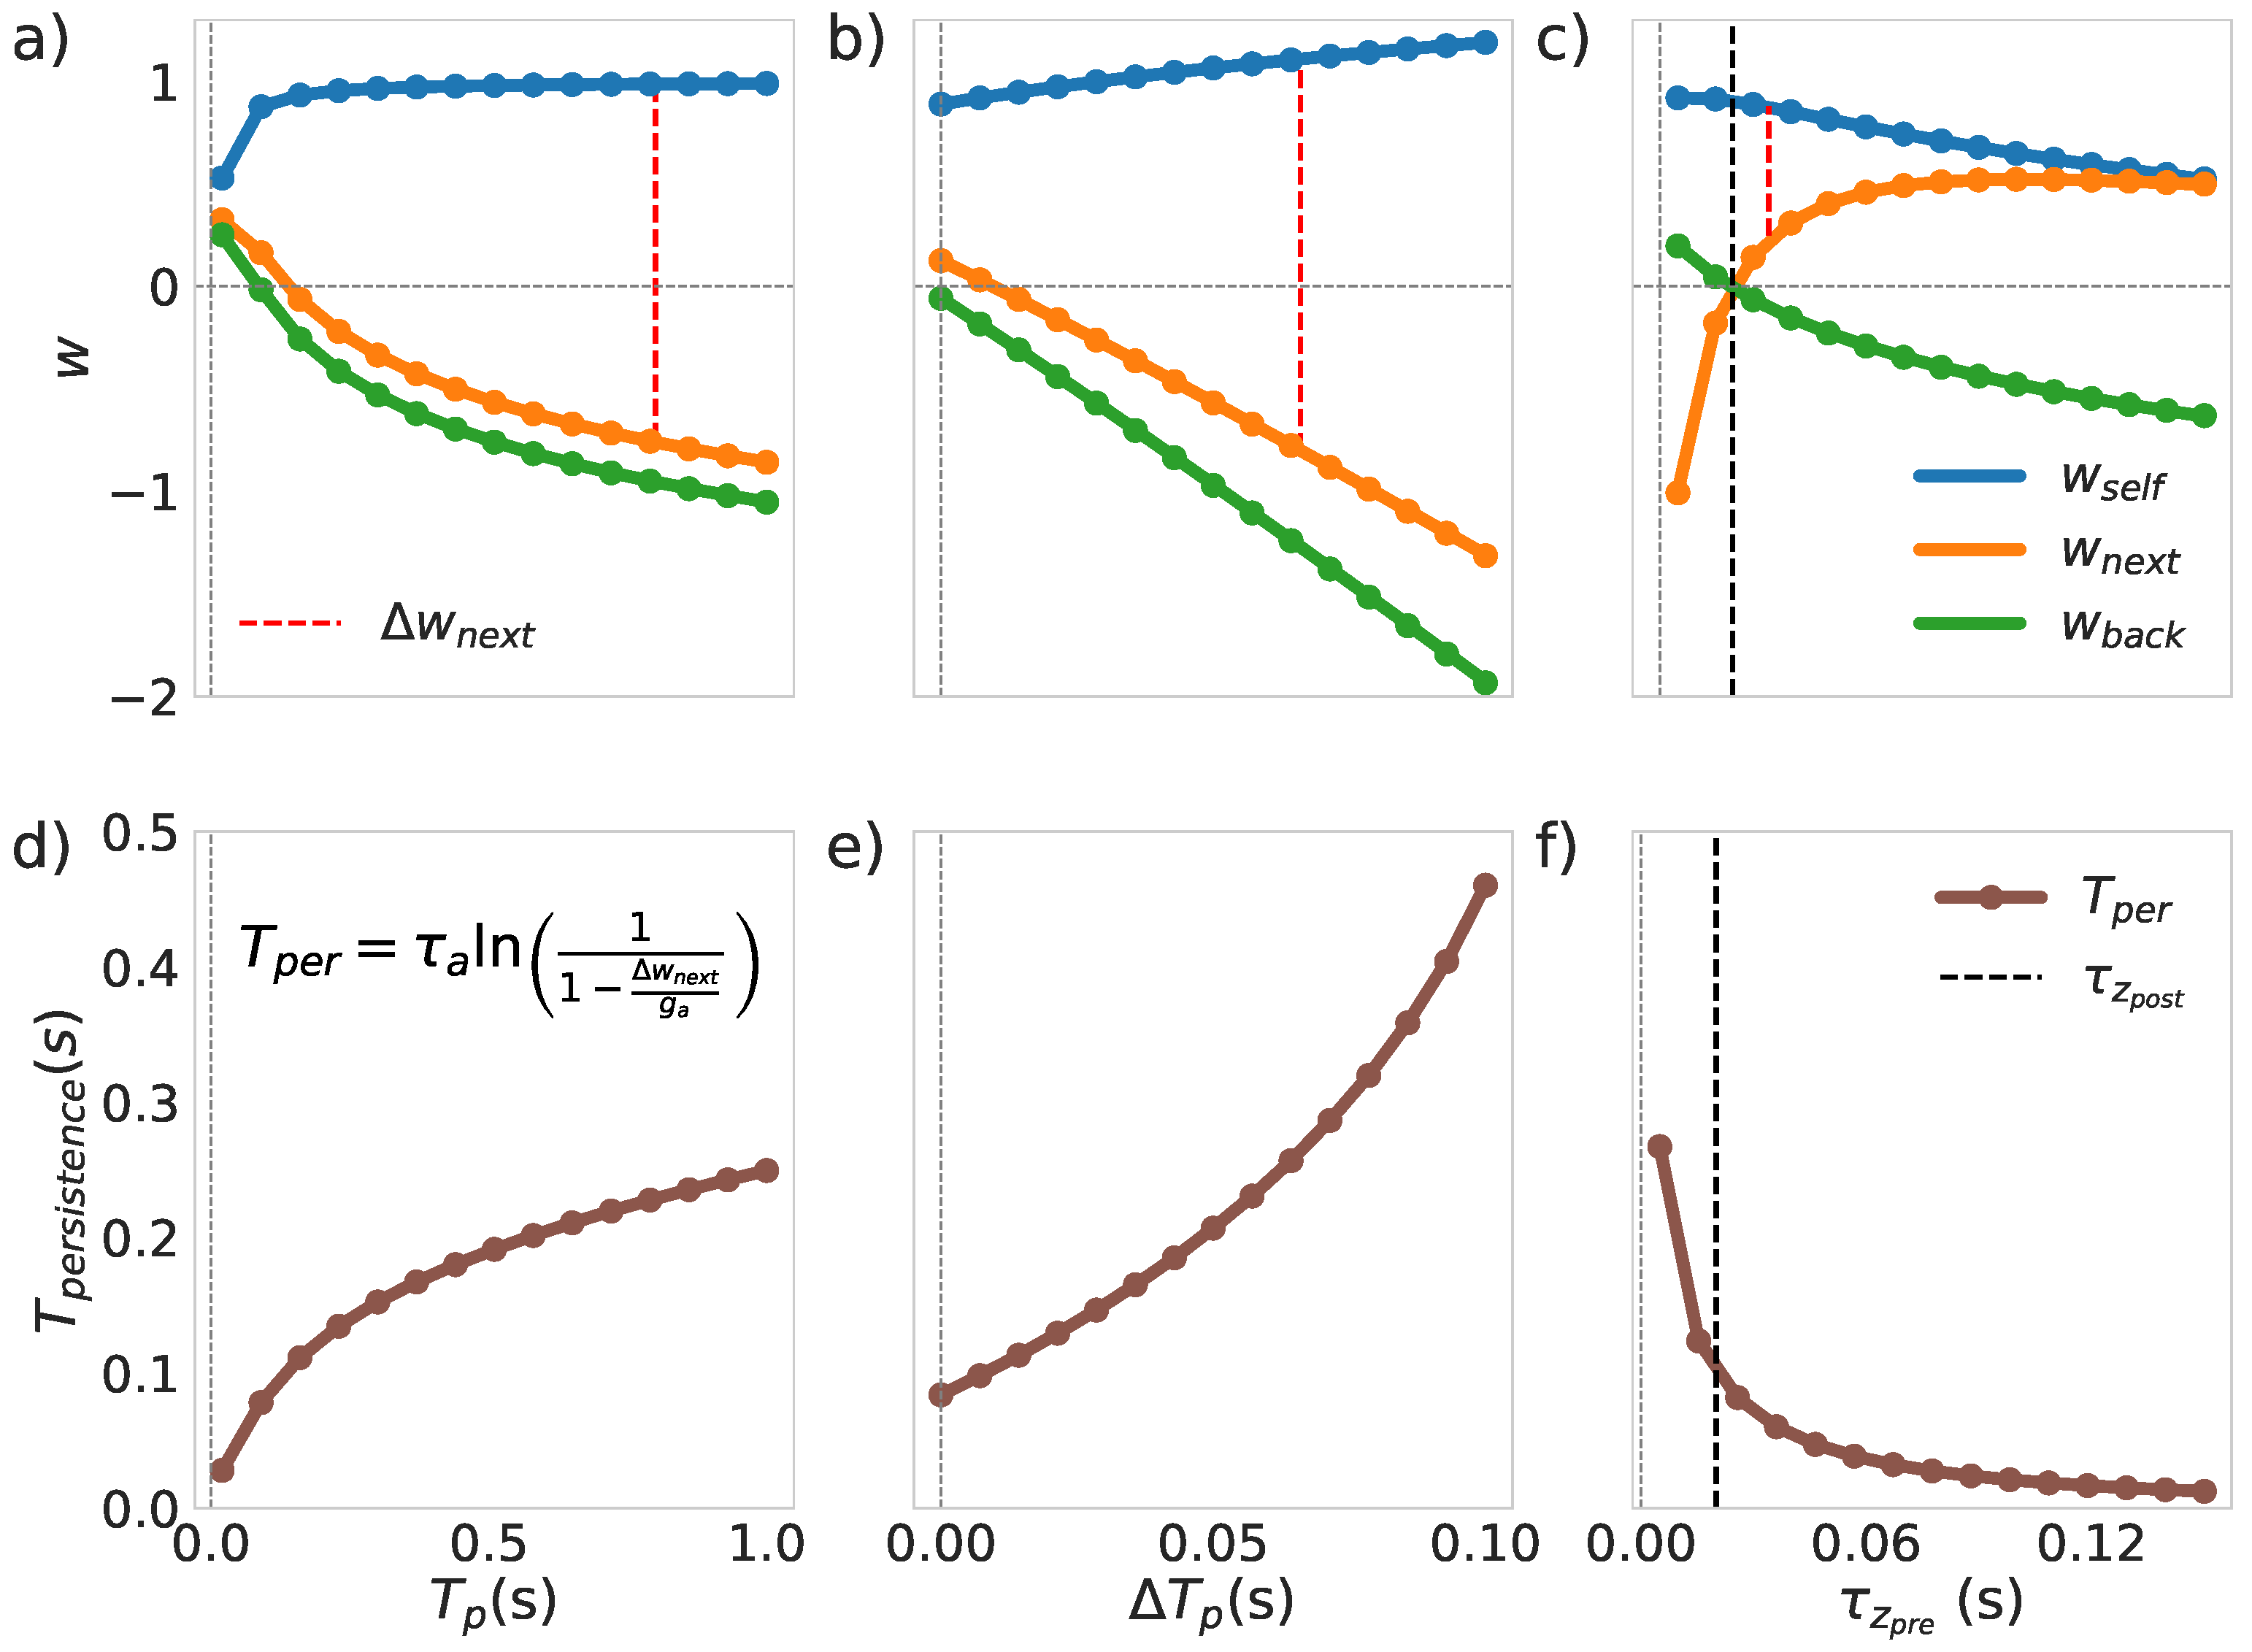
\includegraphics[scale=0.20]{training.pdf}
\caption{Characterization of the connectivity as a function of the training protocol. Here we show how the $w_{self}$, $w_{next}$, $w_{back}$ depend on the training protocol parameters. We also show the effects of training on the persistent time of the attractors $T_{persistence}$. The equation on the inset in d) relates $T_{persistence}$ to   $\Delta w_{next} = w_{self} - w_{next}$ which we show as dashed red line on the top figure. When the parameters themselves are not subjected to variation their values are training time = $100 \, ms$, IPI $= 0 \, ms$, $\tau_{z_{pre}}  = 25 \, ms$, $\tau_{z_{post}}= \, 20 ms$ for all the units. In the following explanation everything that we say about $w_{next}$ can be applied to $w_{back}$ as they are generated with the same process but with a different time constant on their filters. a) we observe that as the training time increases the value of $w_{self}$ quickly stabilizes but the value of $w_{next}$ becomes smaller progressively. This can be explained by the fact that while the self co-activation remains constant with respect to the complete training protocol (stabilizing $w_{self}$) the co-activation between units becomes a smaller portion of the whole training protocol (making $w_{next}$ smaller). This is reflected on d) where we see that $T_{persistence}$ rate of growth becomes constant with bigger training times giving a logarithmic encoding of time.  We see on b) that $w_{self}$ keeps increasing while $w_{next}$ is decreasing with longer IPIs. The longer IPIs bring about an overall longer training protocol which makes the self co-activation more meaningful and $w_{self}$ bigger. $w_{next}$, on the other hand, naturally decreases as a longer IPI makes the co-activation between the units smaller as their activations are father from each other in time. e) we can observe the effect of this dynamic $T_{persistence}$ to increase logarithmicaly with longer IPIs. In c) we can appreciate that the effect of increasing $\tau_{z_{pre}}$ is to make the time coincidence of units in time less important. This is reflected by the fact that $w_{self}$ which reflects the self-activation becomes smaller and that the $w_{next}$ becomes bigger. Note here that when $\tau_{z_{pre}}$ becomes bigger than $\tau_{z_{post}}$ (marked with a dashed red line) coincides with $w_{next}$ becoming bigger than $w_{back}$ as we should expect. We can observe also that  $\Delta w_{next}$ becomes almost zero for big values of $\tau_{z_{pre}}$ which is reflected on f) as smaller and smaller values for $T_{persistent}$. }
\label{fig:training}
\end{figure}

\subsection{Noise}

\begin{figure}[H]
\centering
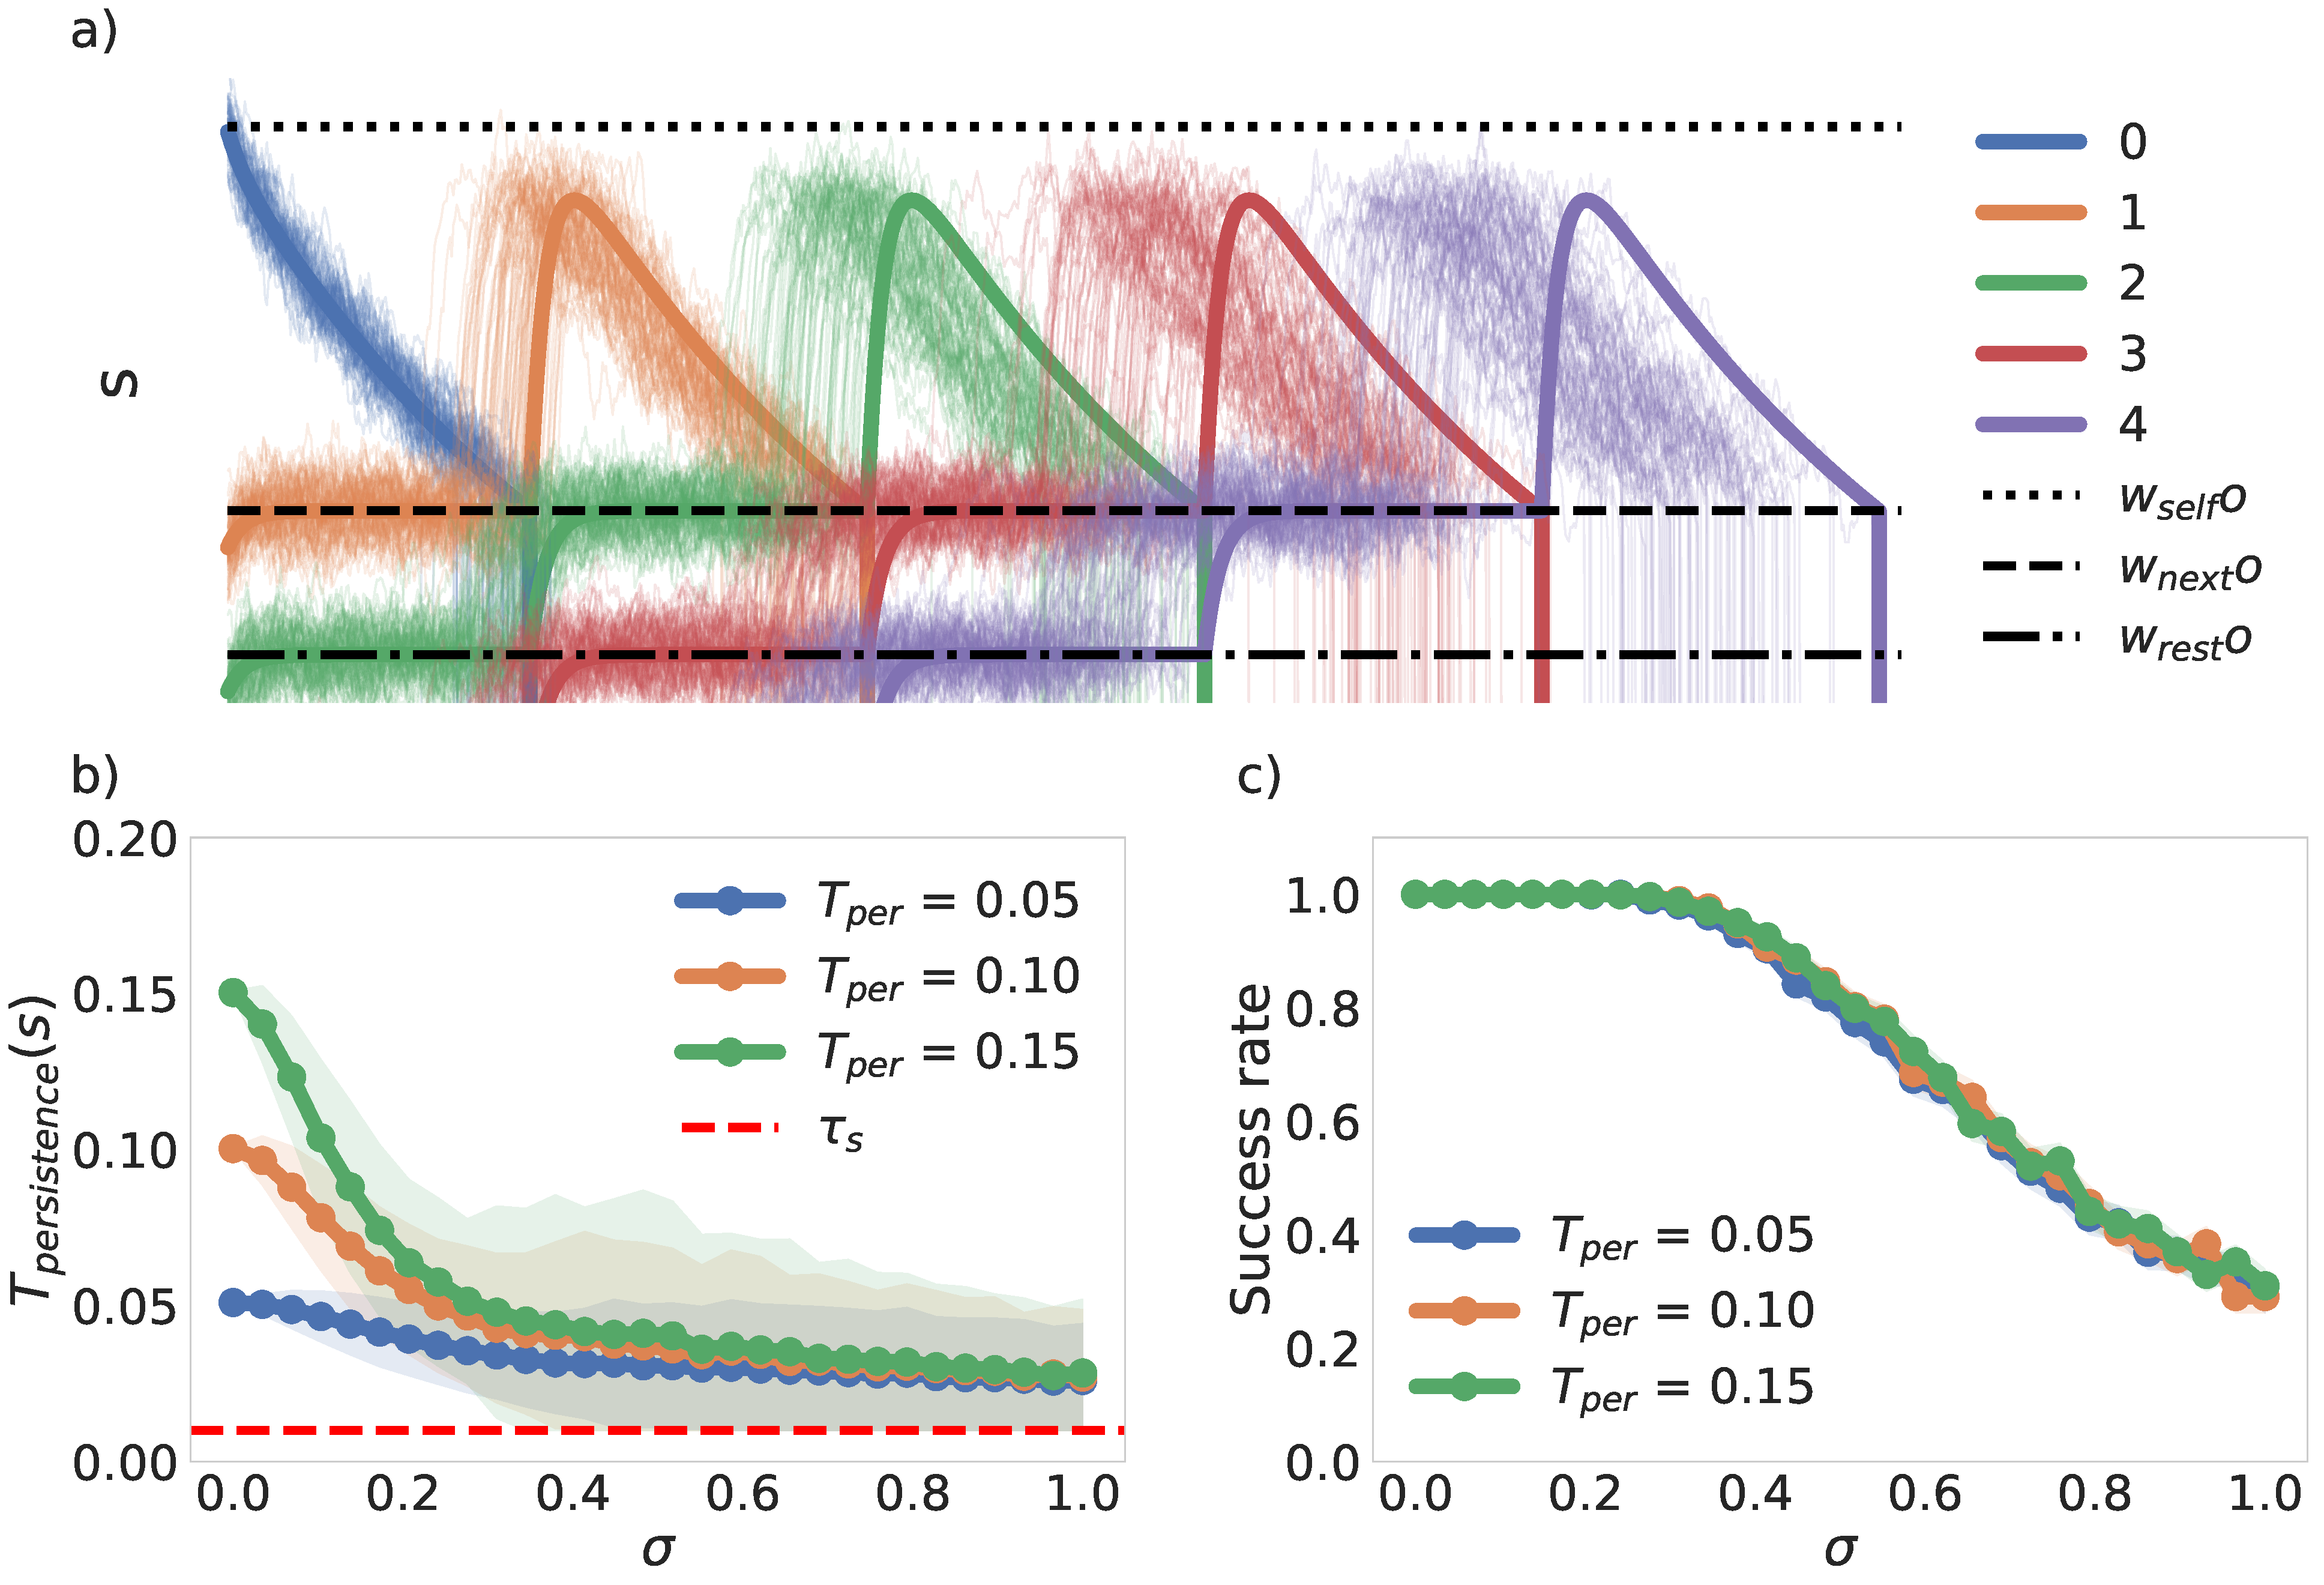
\includegraphics[scale=0.17]{noise_diagram.pdf}
\caption{Effects of noise in trajectories and persistent time. a) we show here an example of noisy trajectories as they evolve in time. The solid lines indicate the deterministic trajectories the system would follow in the zero noise case. In dotted, jagged and dashed lines we depict the important landmarks of connectivity $w_{self}$, $w_{next}$ and $w_{rest}$ respectively. We can notice that in the noisy case the units make the transition to the next unit faster that they would have done in the deterministic case as illustrated more clearly on the red and purple lines that fall far behind their deterministic counterpart. We characterized this phenomena more systematically bellow b) where we show that even if the success vs noise profile is not affected by variations $T_{persistence}$ we can also observe in c) that the mean value of $T_{persistence}$ quickly decays with noise.}
\label{fig:noise_scheme}
\end{figure}

\begin{figure}[H]
\centering
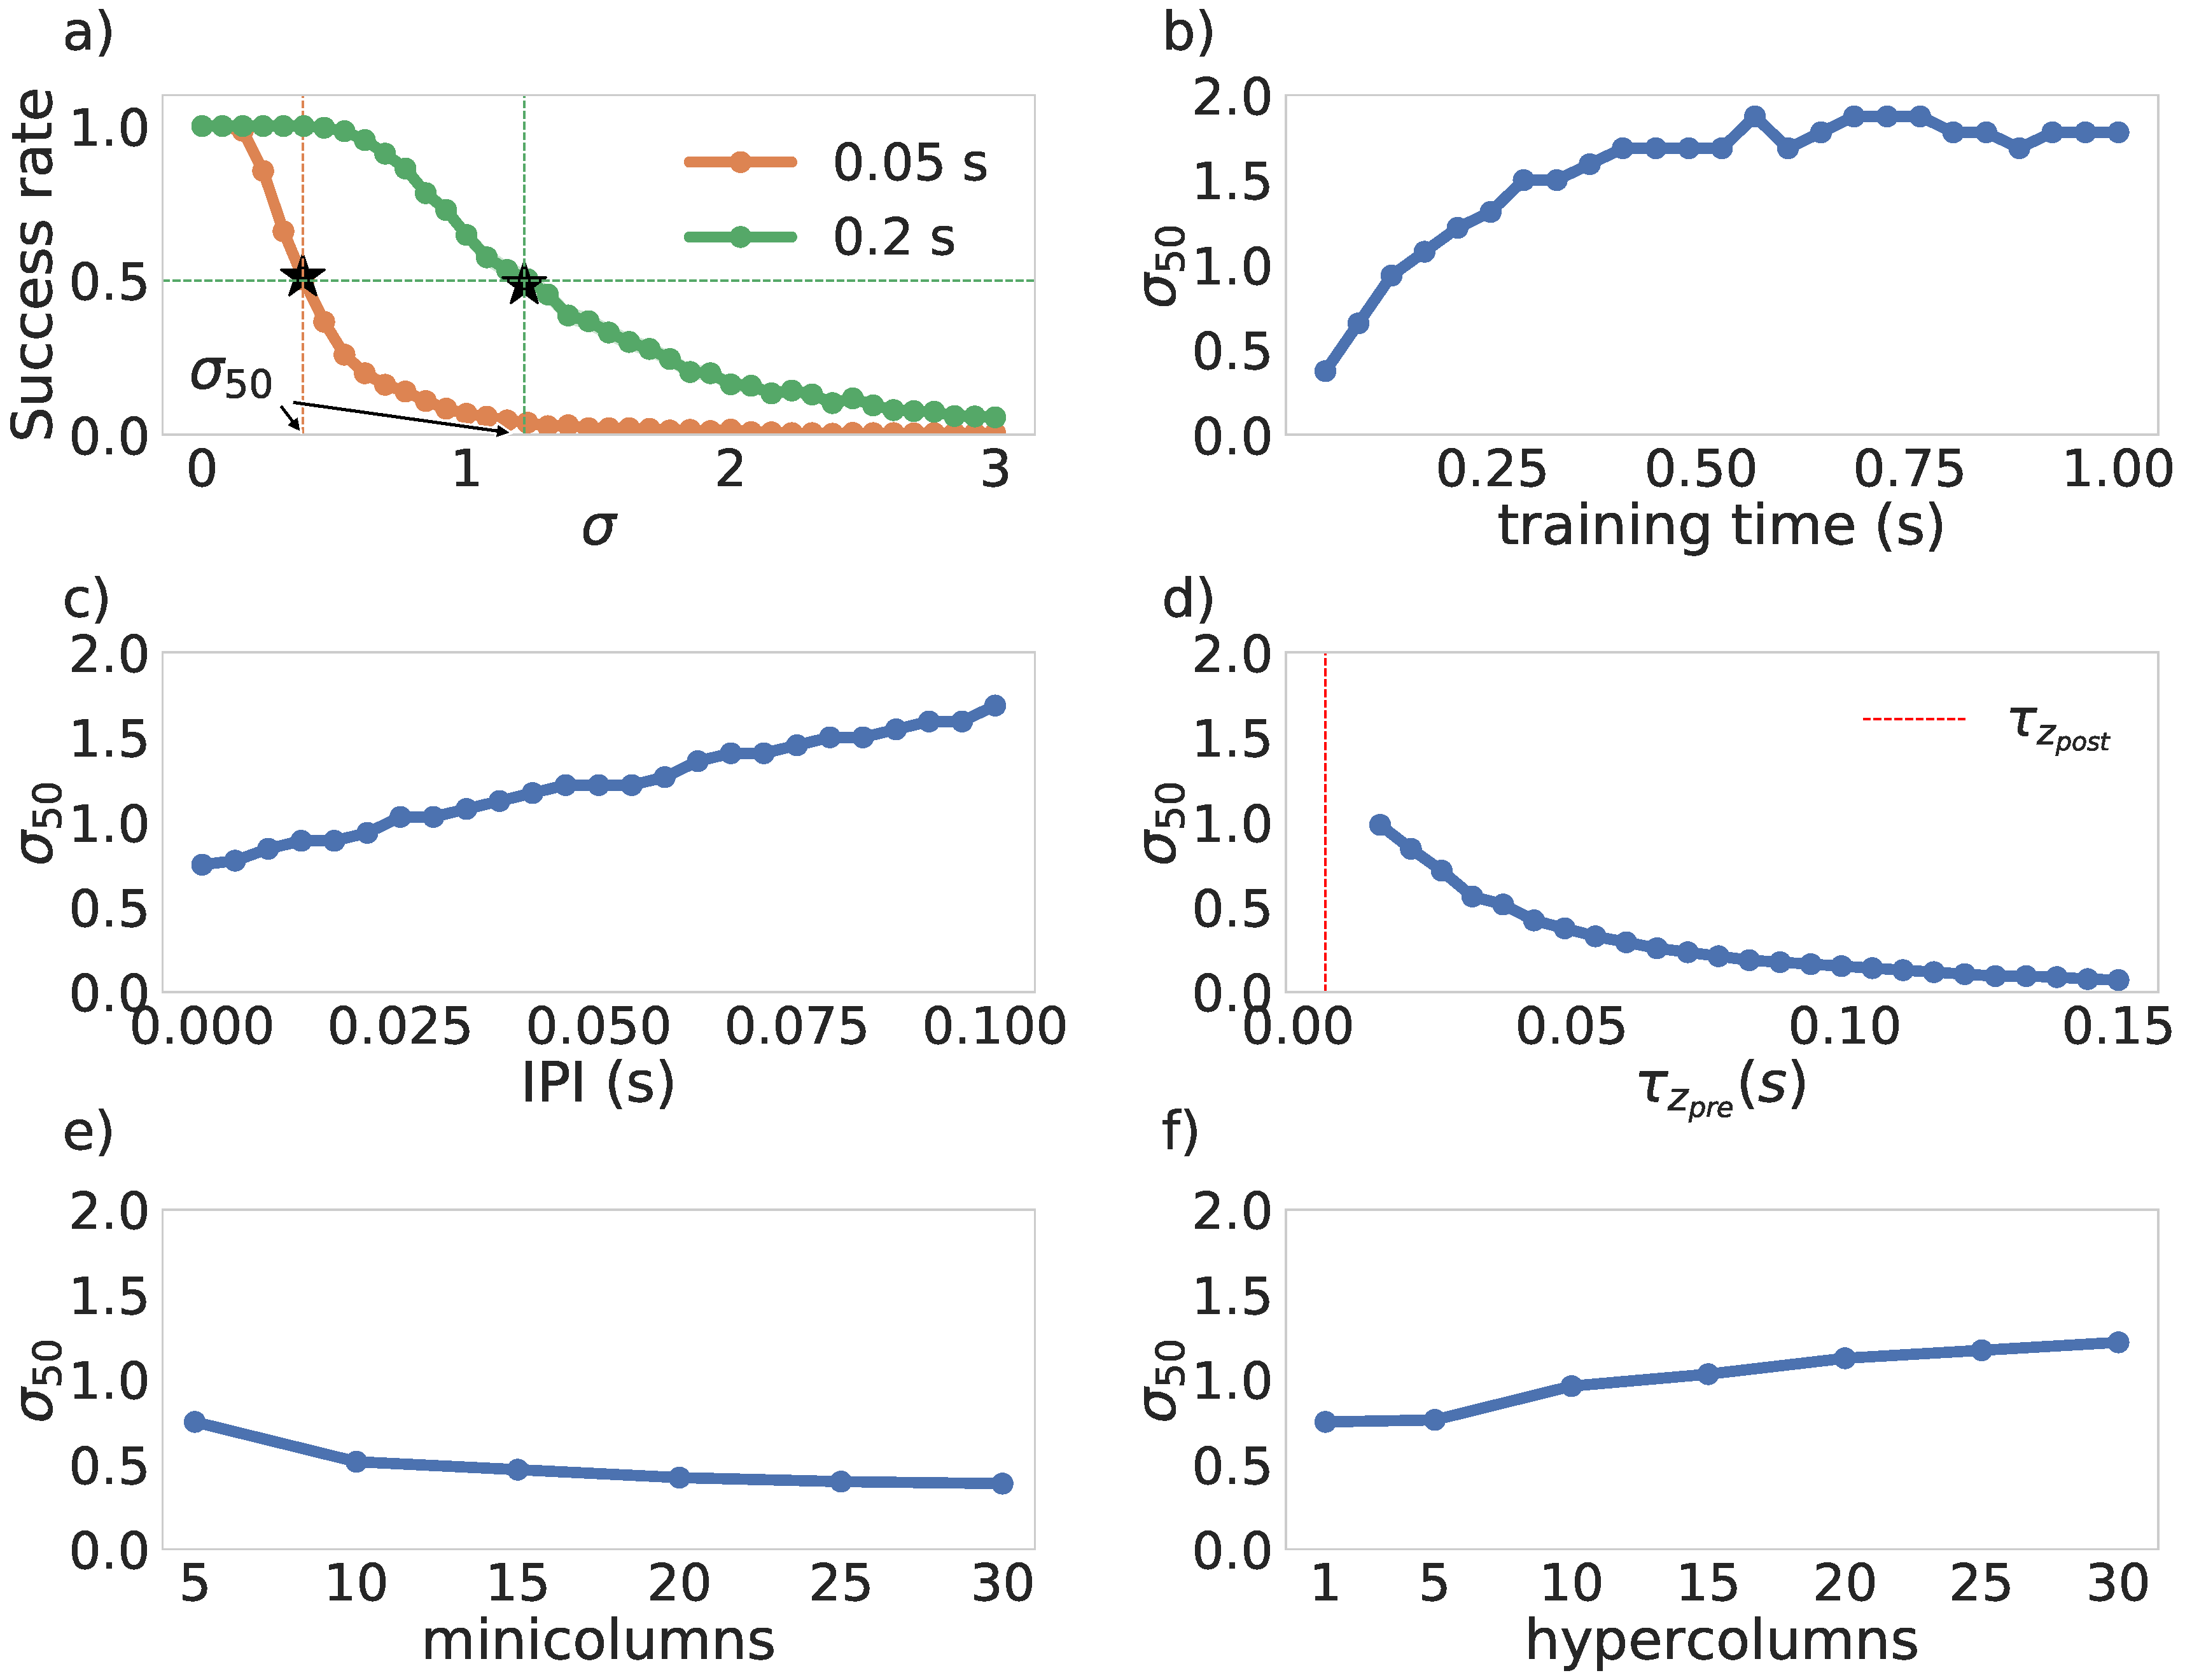
\includegraphics[scale=0.20]{noise_robustness.pdf}
\caption{We characterized  how robust the networks that we train are to noise in their recall phases.  We use the following parameters for all the training except when the parameter itself was varied: training time $= 100 \: ms$, IPI $= 0 \: ms$, $\tau_{z_{pre}} = 25 \: ms$, $\tau_{z_{post}} = 20 \: ms$ minicolumns $=5$, hypercolumns$=1$. a) Two examples of the success vs noise profile for two neural networks ($50 \: ms$ and $200 \: ms$. We also annotated in black the points at which noise level the probability reached its half value, we denote the arguments of such value $\sigma_{50}$. Note that the bigger $\sigma_{50}$ is the more robust the system is to noise and vice versa. Using this fact we use $\sigma_{50}$ quantify the variation of robustness with the training parameters. b) $\sigma_{50}$ with respect to training, we can see that the system becomes more robust the longer it is trained as this increases the distances between the weights, we can see the same effect on c) where the separation of weights produced by longer $IPI$ leads to the same outcome. The opposite effect is observed on d) where the system becomes less robust with longer $\tau_{z_{pre}}$, which we can explain by appealing to the fact that this also makes the weights closer in distance. We also show in e) that the sequence becomes less robust the longer it is, this can be explained by thinking on every link on the chain as a point of failure on itself. Naturally, adding more links to the chain makes it more likely to fail at some point. Finally, in f) we show that there is a strong scaling effect with the number of hypercolumns. We believe this effect is due to creating more robust representations where if a wrong transition occurs at a unit of some pattern the attractor effect of the remaining units of the pattern will correct for the local mistake.}
\label{fig:noise_sensitivity}
\end{figure}


\subsection{Representations}

\begin{figure}[H]
\centering
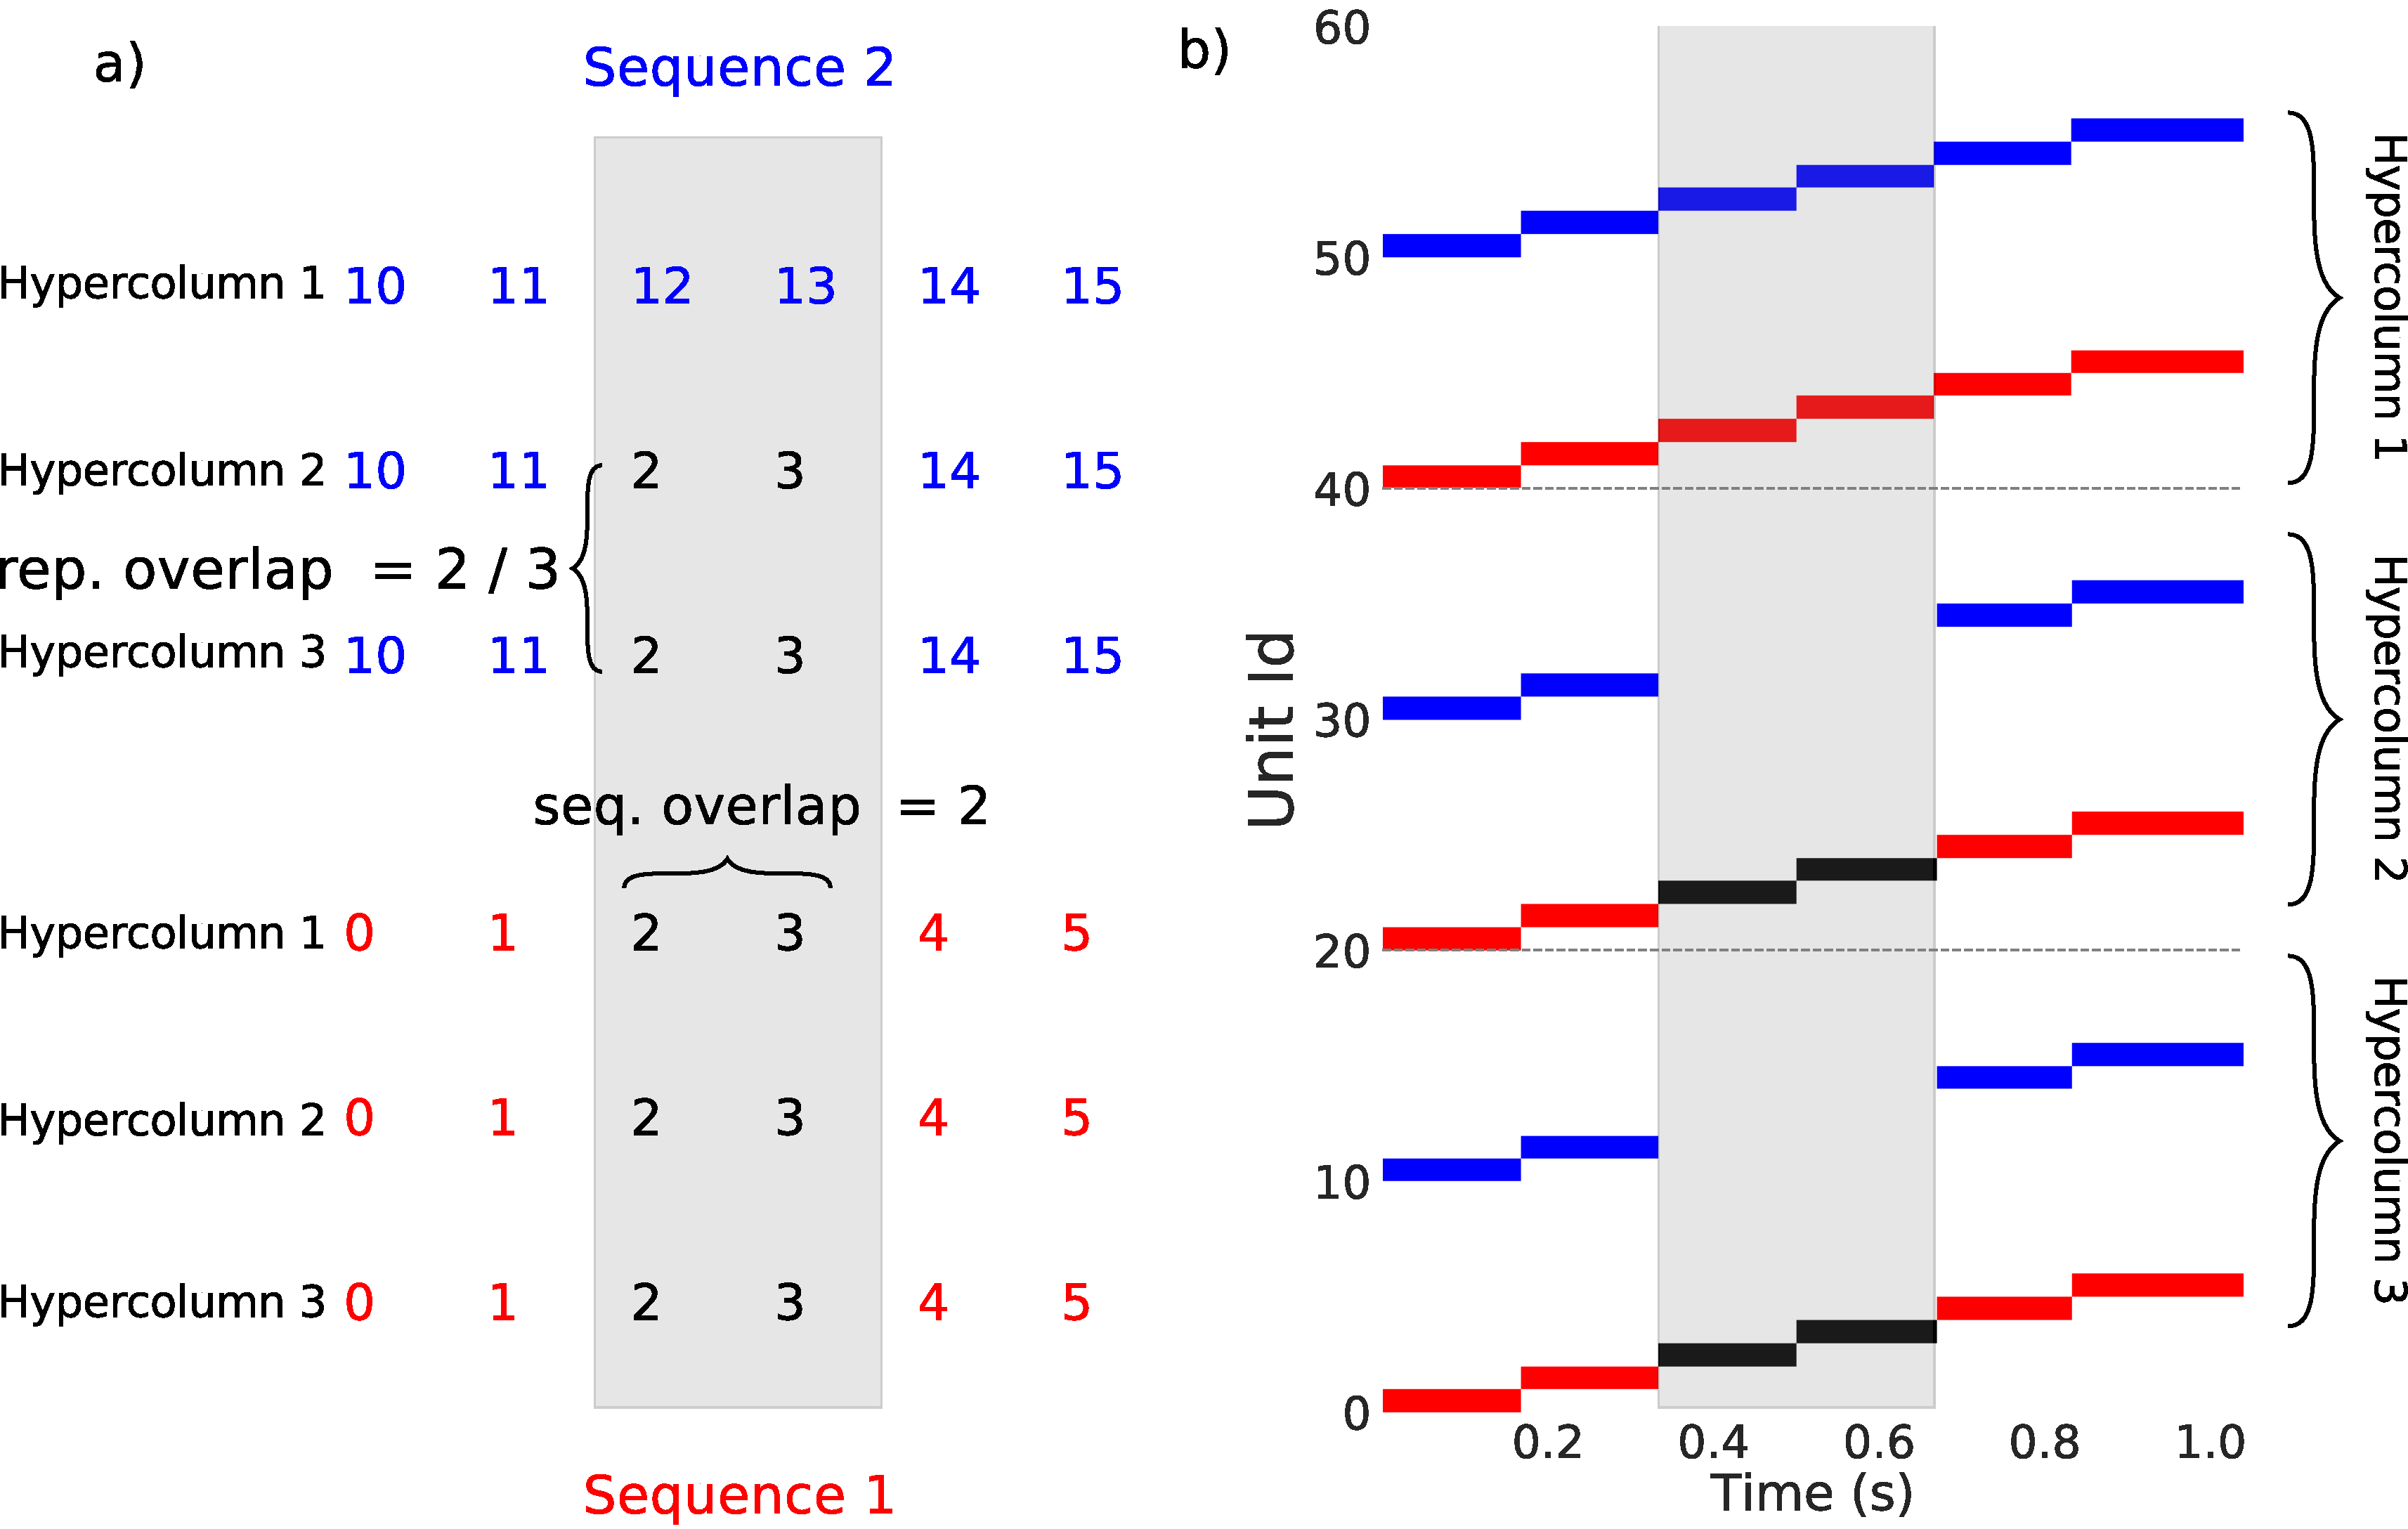
\includegraphics[scale=0.20]{rep_diagram.pdf}
\caption{Two sequences, red and blue, with some overlap in their representations. a) A symbolic representation of the sequences, where each row is a hypercolumn and each column a pattern. The single entries represent the particular unit that was activated. If we pay attention to the gray area we can observe that the second and third hypercolumns of the second sequence share the same units activated with the first sequence (units 2 and 3). We say that the sequences have a representation overlap of $p=\frac{2}{3} = \frac{\text{\# hypercolumns shared}}{\text{\# total hypercolumns}}$. If we look at the sequence as a whole we see that the patterns where those representations are shared are 2 of the 6 patterns in the sequence, we say that the the sequences have a sequential overlap of 2. b) We show here the superposition of the recall phase for both sequences with each sequence recall emphasize by its color. We can appreciate inside the gray area that the second and third hypercolumns have the same units activated (depicted in black) at the same point in the sequence reflecting again a representation overlap of $\frac{2}{3}$.}
\label{fig:rep_diagram}
\end{figure}

Disambiguation task parameters.
When the parameters are not subjected to variation themselves their values are training time $= 100 \: ms$, IPI $= 0 \: ms$, $\tau_{z_{pre}} = 25 \: ms$, $\tau_{z_{post}} = 20 \: ms$ minicolumns $=20$, hypercolumns$=10$,  

\begin{figure}[H]
\centering
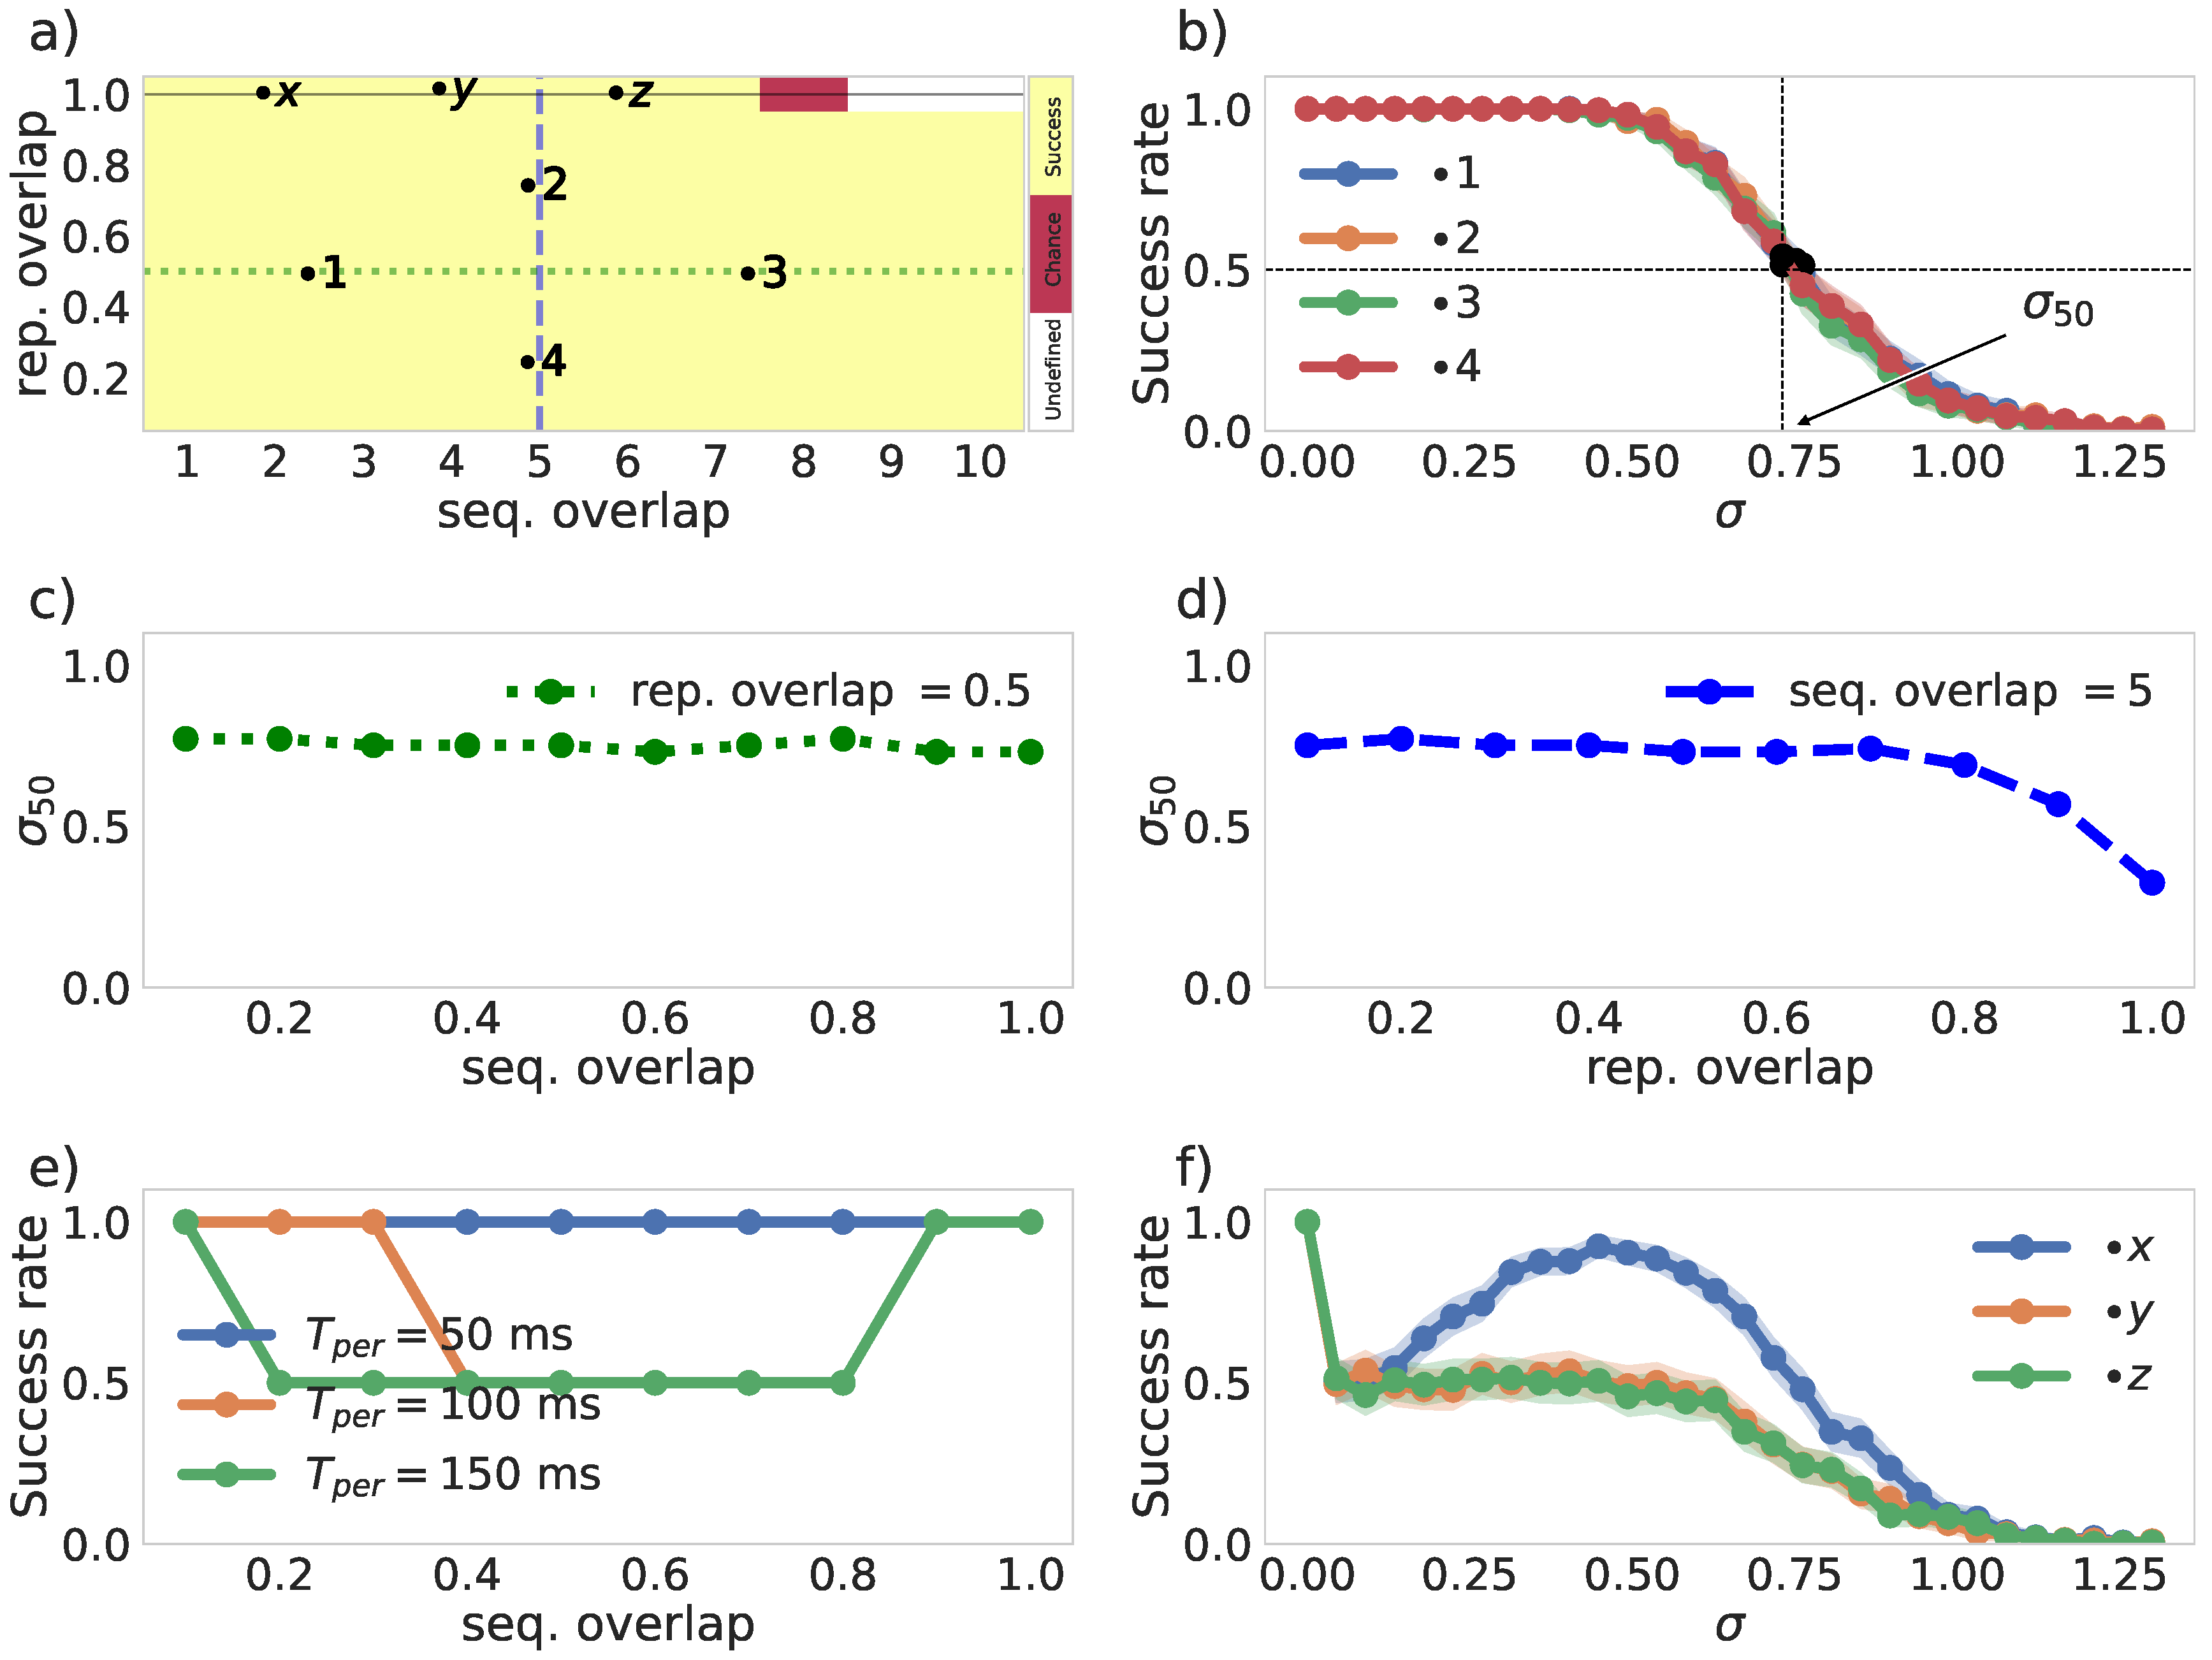
\includegraphics[scale=0.20]{representations.pdf}
\caption{A characterization of the different overlap conditions. a) We test whether we get correct recall for the two sequences in the zero noise condition. Besides the disambiguation regime where the overlapped patterns are completely identical the network can successfully recalled overlapped sequences over a wide arrange of sequential and representation overlap parameters b) To test whether our results are robust to noise we show the profile of the success rate vs noise of the four numbered black points in a) (1, 2, 3, 4). The profiles overlap completely each other which indicate 1) that the system is robust to noise and 2) that this robustness property is not very sensitive to changes on the overlap parameters. To offer a more systematic proof of this fact we  characterize the $\sigma_{50}$  (indicated by an arrow on b ) parameter along the dashed lines on 1. c) $\sigma_{50}$ variation with sequence overlap (green dashed line in a). f) $\sigma_{50}$ variation with representation overlap (blue dashed line in a). e) As the disambiguation capabilities of the network are mediated by memory (here capacitive effects mediated by $\tau_s$) it is to be expected that the longer the temporal overlap of two sequences the harder it is for the network to solve the disambiguation tasks. In order to illustrate this effect we show how the successful disambiguation along the disambiguation line (black line in a)) depend on the encoded persistent time of the sequences $T_{persistence}$. Even if the system can solve the disambiguation scenario successfully for small values of $T_{persistence}$  the effect is not very robust to noise  as we show in f) where we depict the success vs noise profile for the three numbered black points in  a) (a, b and c). First, it is to note that even a small amount of noise degrades the system to chance level recall (0.50). Second, we have a resonance phenomena for low levels of sequential overlap, this can be explained with the fact that the noise effectively reduces the mean $T_{persistence}$ which makes the disambiguation power of the network strong enough to even overcome the noise.}
\label{fig:representations}
\end{figure}


\subsection{Non-homogeneous training conditions}

\begin{figure}[H]
\centering
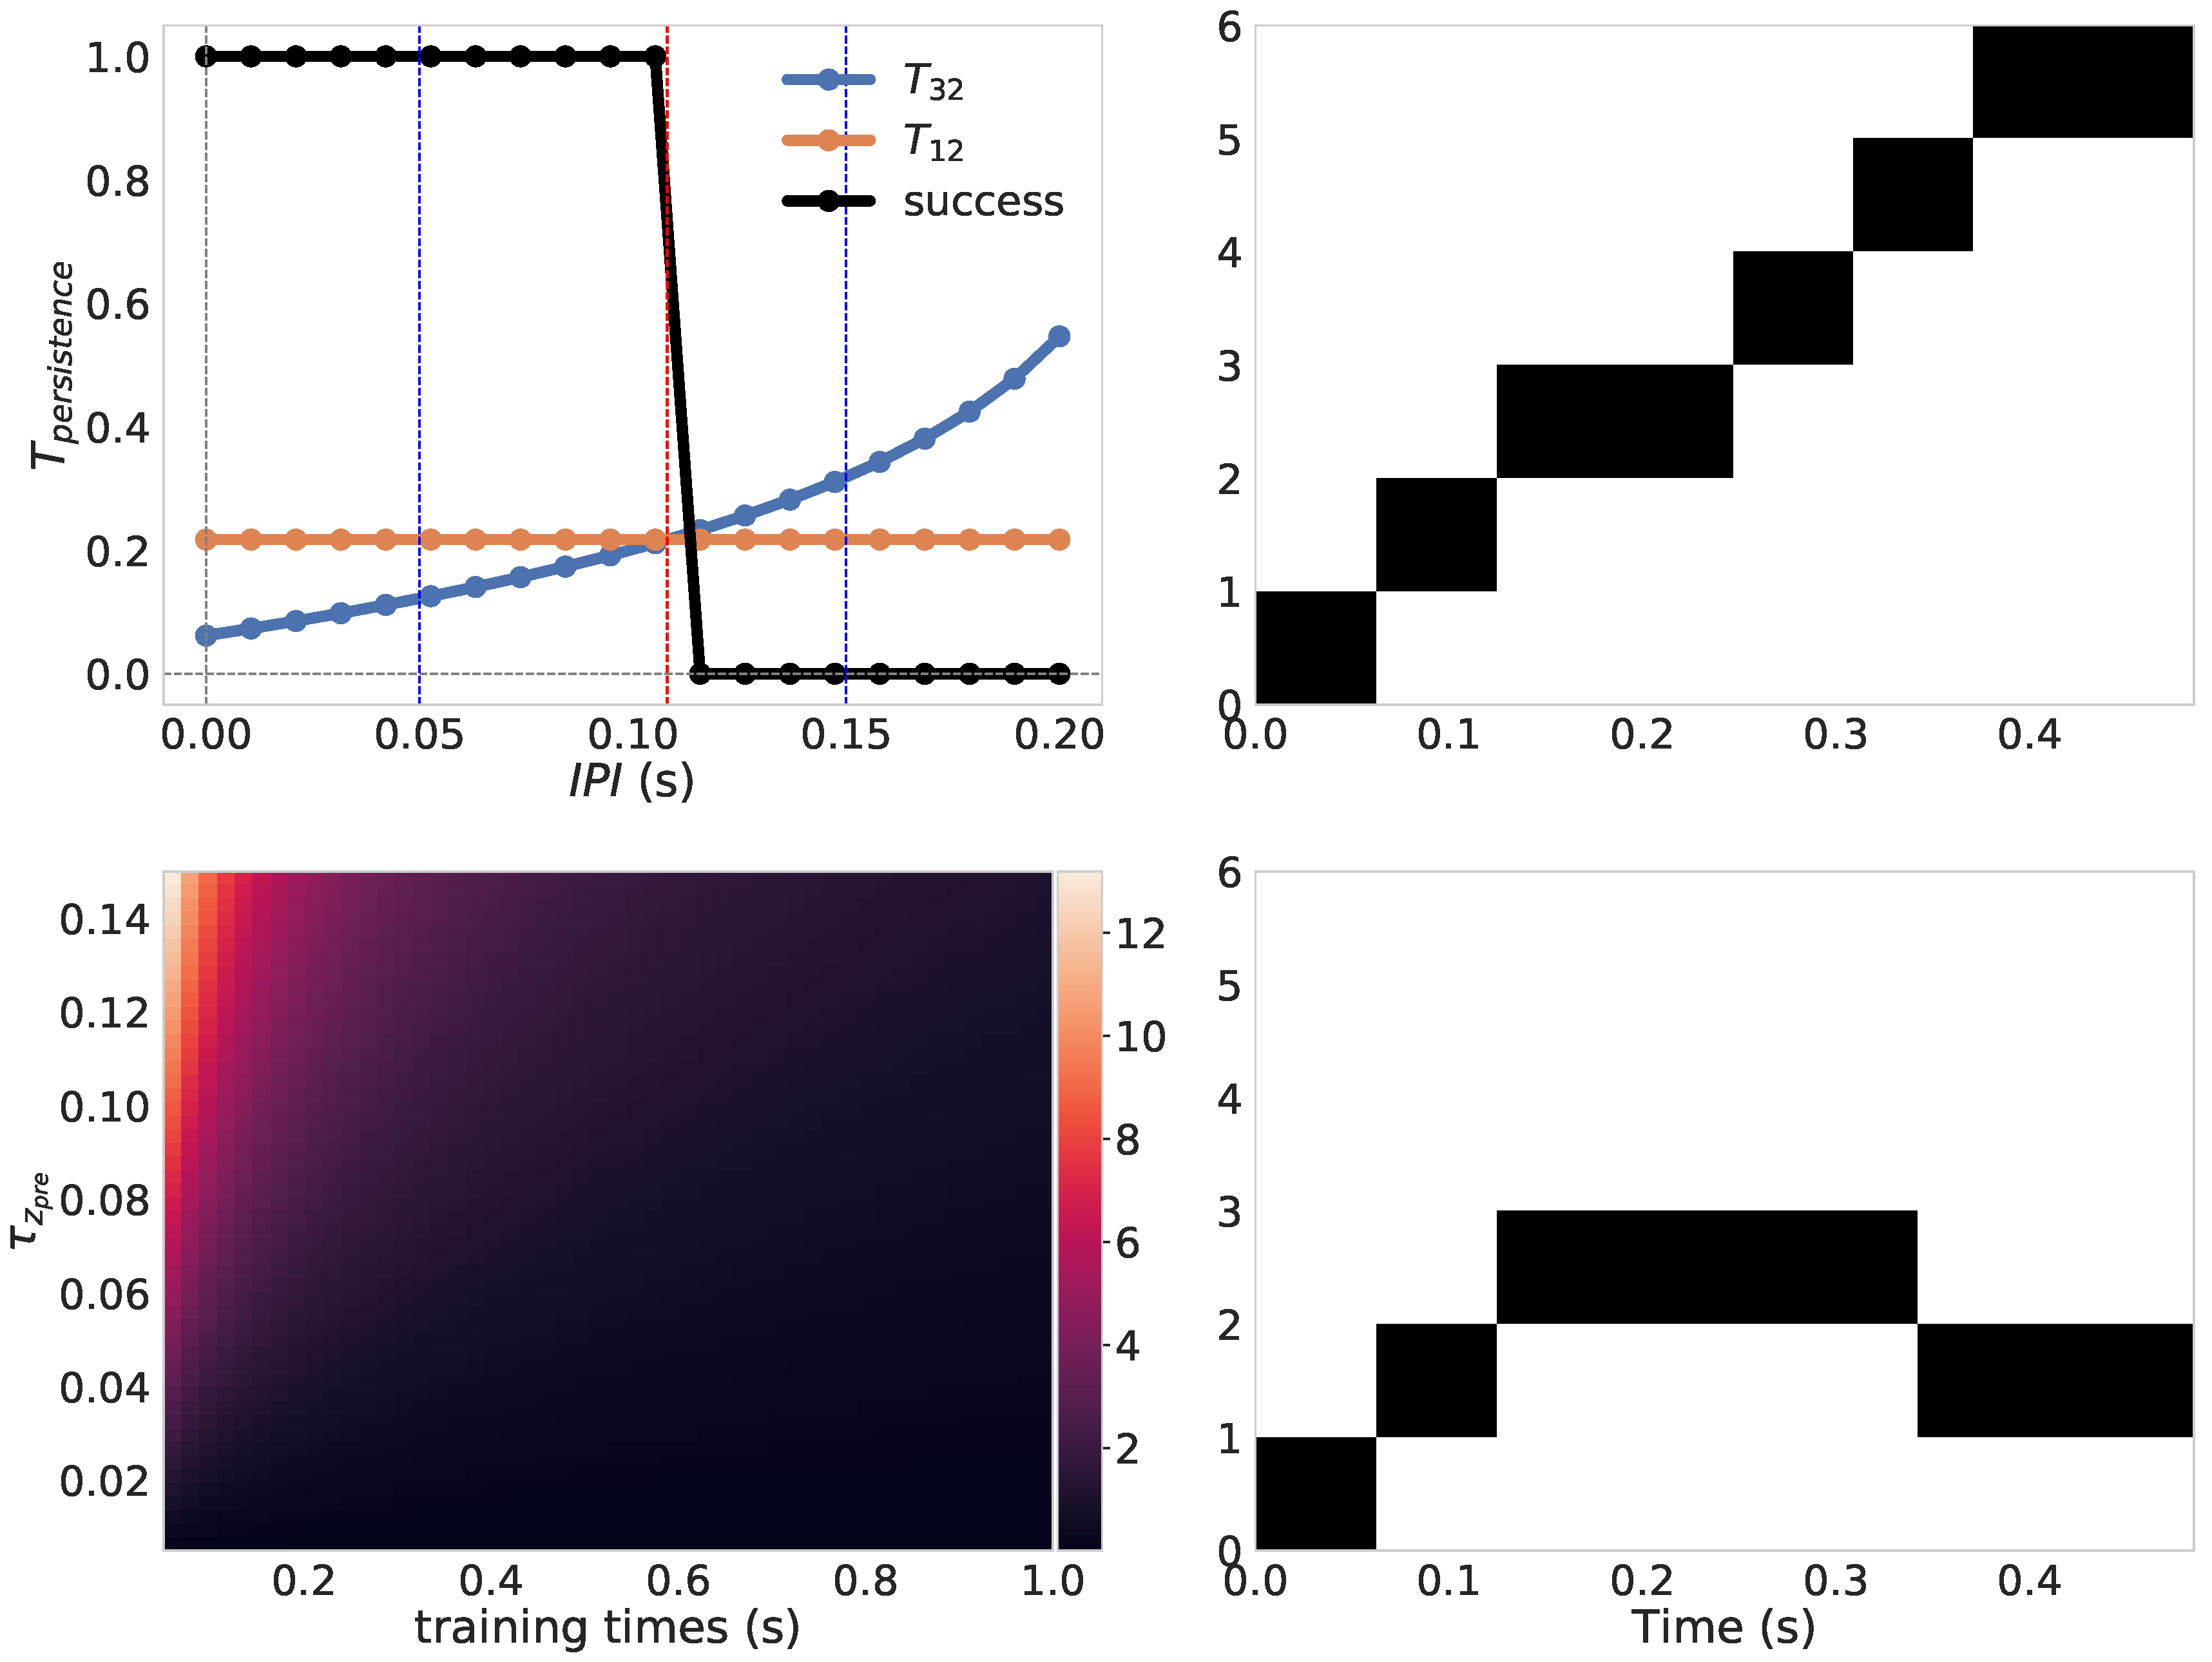
\includegraphics[scale=0.20]{ipi_non_homogenous.pdf}
\caption{A characterization representational and sequential overlap. a) }
\label{fig:non-homo}
\end{figure}

\section{Methods}

\subsection{Pattern Activation}
We define pattern activation in the following way. First we calculate a vector with the cosine similarity between all the patterns stored and the network state $\mathbf{o}$ at every point in time $sim_i(t) = \frac{\mathbf{pattern_i} \bullet  \mathbf{o}(t)}{\Vert \mathbf{pattern_i} \Vert \Vert \mathbf{o}(t) \Vert}$. Note that this will give a time series for every element of the vector $sim$. Second we form a times series with the most similar pattern to the network state at every point in time by choosing the pattern index with the most similarity $winner(t) = \max \: \mathbf{sim(t)}$. This time series is as long as the number of points in time that the simulation possess. Finally, in order to get the sequence of activations we considered as active any pattern that was the winner for longer than  $T_{winning} \:$ which was set to $T_{winning} = \tau_s = 10.0 \: ms$ unless otherwise specified.   

\subsection{Recall Protocol}
For the recall protocol we briefly activate the complete pattern for $\tau_s = 10 \: ms$. The network is then free to evolve according to its internal dynamics. The sequence (0, 1, 2, 3) is considered to be correctly recalled if by activating the first pattern in it (pattern 0) all the others patterns on the sequence are activated in the specific order that they were stored. Given that for many possible tasks it suffices that the network state ends in the correct pattern or that only a part of the sequence is recalled correctly our success criteria may appear overly narrow. However in making this choice we have traded generality for specificity with the aim of establishing a lower bound for the correct recall conditions of sequence processing.


\subsection{Calculation of Persistent Time}
In order to calculate $T_{persistence}$ of pattern $i$ we calculated the difference between the time $t_1$ at which pattern $i$ became activated ($winner(t_1) = i$) to the first point in time at which it was not ($winner(t_2) \neq i$). Then we simply defined $T_{persistence} = t_2 - t_1$.

As shown in equation \ref{eq:persistent_times} the persistent time depends on both the weight and bias differences $\Delta w_{next} = w_{self} - w_{next}$ and $\Delta \beta = \beta_{self} - \beta_{next}$ and the adaptation gain $g_a$. This allow us to  set the persistent time of an attractor to any desired value by adjusting the adaptation gain with the formula $g_a = \frac{(\Delta w_{next} + \Delta \beta)(1 - r)}{1 - r - e^{\frac{T_{persistence}}{\tau_a}}}$. We use this adjustment to control for $T_{persistence}$ after training in order to decouple the effects of training from the ones of the persistent time in the recall phase. 

\subsection{Training Protocol}
For our training protocol we created a time series  $\mathbf{s}(t)$ to represent the input. $\mathbf{s}(t)$  encodes the information about the training time and the inter-pulse interval. We then performed off-line batch learning of the parameters using the integral formulation of the training equations above.

\begin{align}
z(t) &= \frac{1}{\tau_z } \int_{-\infty}^{t} s(\tau) e^{-\frac{t - \tau}{\tau_z}} d\tau \label{eq:flitering}  \\
p_i(t) &= \frac{1}{t}\int_0^{t} \underset{post}{z_i}(\tau) d\tau  \label{eq:bcpnn_off_line_prob} \\
p_{ij}(t) &= \frac{1}{t}\int_0^{t} \underset{post}{z_i}(\tau) 
\underset{pre}{z_j}(\tau) d\tau \label{eq:bcpnn_off_line_joint} 
\end{align}

Where we have calculated two $z$ traces, one for $\tau_{z_{pre}}$ and the other for $\tau_{z_{post}}$. The limits of the integrals were selected to coincide with the total duration of all the input. After we have the values of the probability traces we calculated $w$ and $\beta$ by using the BCPNN rule in equation \ref{eq:bcpnn}.

For training the two sequences with the overlapped representations we created a time series with the sequences in succession but separated among them by $1s$. This ensured the training protocol were uncoupled from each other.



\subsection{Noise}
We added noise in the system as an injection of white noise with variance $\sigma_{in}$ into the system at every time step. However, we characterized the system in terms of the steady state standard deviation that the system would have it it was an Ornstein–Uhlenbeck (OU) process given by $\sigma_{out} = \sqrt{\frac{\tau_s}{2}} \sigma_{in} \sim 0.07 \sigma_{in}$. The rational behind this choice is that $\sigma_{out}$ will be the actual standard deviation that the current $s$ in equation \ref{eq:current} will be subjected to precisely this standard deviation. It is important to say that thanks to the separation of times scales ($\tau_s \ll \tau_a$) the system behaves mostly as an OU process and is only the winner-take-all dynamic around the transition points that deviates the system from it as it can be appreciated in figure \ref{fig:noise_scheme}a). Throughout this work we use $\sigma = \sigma_{out}$ unless otherwise stated. 

We calculated the success rate by simply averaging how many of a given number of trials successfully recalled the sequence. In order to quantify the uncertainty over our estimates for the success rate for different degrees of noise we utilized the Wald method to provide the $95 \% $ confidence intervals for the success rate estimates:

\begin{align} 
\hat{p} \pm 1.96\sqrt{\frac{\hat{p}(1 - \hat{p})}{N_{obs} }} \label{eq:confidence}
\end{align}

For this work we mostly used $N_{obs}=1000$ and therefore we have approximately $\hat{p} \pm 0.0134$ or deviations of $1 \%$.  


\subsection{Calculation of Noise Sensitivity}
In order to systematically characterize how different parameters of our training protocol affect the sensitivity of the resulting network to noise we calculated $\sigma_{50}$. We defined $\sigma_{50}$ as the  value of $\sigma$ for which the probability of correctly recalling a given sequence is $\frac{1}{2}$. Finding such $\sigma$ is a instance of the Stochastic Root Finding Problem \cite{pasupathy2010choosing}. To estimate this we have used the naive bisection algorithm for deterministic functions by using the averages as estimates of the actual values. We stopped the algorithm as soon as the success rate corresponding to our estimate of $\sigma_{50}$ was contained in the Wald confidence interval as presented in \ref{eq:confidence}. As a validation of the algorithm ability to find the  correct value we calculated the success rate that we found at $\sigma_{50}$ as we show ther figure \ref{fig:noise_calibration} of the appendix. We find that the algorithm consistently finds a value of $\sigma_{50}$ that fulfills the criteria of the success rate being $\frac{1}{2}$. That said, in order to find a more standard statistical measure of the error in $\sigma_{50}$ we would require to perform an amount of estimations of $\sigma_{50}$ that surpasses our current computational capabilities. We believe though that the purpose of estimating the overall way in which the noise sensitivity depends on the training protocol is accomplished by our method. 

In figure \ref{fig:appendix_noise_sensitivity} in the appendix we also characterized the variation of $\sigma_{75}$ and $\sigma_{25}$  in order to have a more thorough analysis. The trends overall agree with the analysis in figure \ref{fig:noise_sensitivity}.  




\section{Apendix}
\subsection{Analytical solution}
We can solve the deterministic equations analytical with the method of undetermined coefficients. There are two conditions, the unit that is active, and the unit that is not. 


\begin{align*} 
s(t) &= I_{fix} - g_a\left(\frac{C_{charge}}{1 - r} \right) e^{-\frac{t}{\tau_a}} + \left(s_0 - I_{fix} + g_a \left( \frac{C_{charge}}{1 - r}\right)\right)e^{-\frac{t}{\tau_s}} \\
\underset{acti}{s(t)} &= \beta + w - g_a + g_a \left(\frac{1 - a_0}{1 - r}\right) e^{-\frac{t}{\tau_a}} + \left(s_0 - \beta - w + g_a - g_a \frac{1 - a_0}{1 - r}\right) e^{-\frac{t}{\tau_s}}  \\ 
\underset{inact}{s(t)} &= \beta + w - g_a \left( \frac{a_0}{1 - r} \right) e^{-\frac{t}{\tau_a}} + \left(s_0 - \beta  - w  + g_a \left( \frac{a_0}{1 - r} \right) \right) e^{-\frac{t}{\tau_s}} 
\end{align*}

Where $r=\frac{\tau_s}{\tau_a}$ and $C_{charge}=a_0$ for the non-active case and $C_{charge} = a_0 - 1$ for the active case. Same for $I_{fix}=\beta + w$ for the non-active case and $I_{fix} = \beta + w - g_a$ for the active case. 

\subsection{Role of the z-traces' Time Constants}
\begin{figure}[H]
\centering
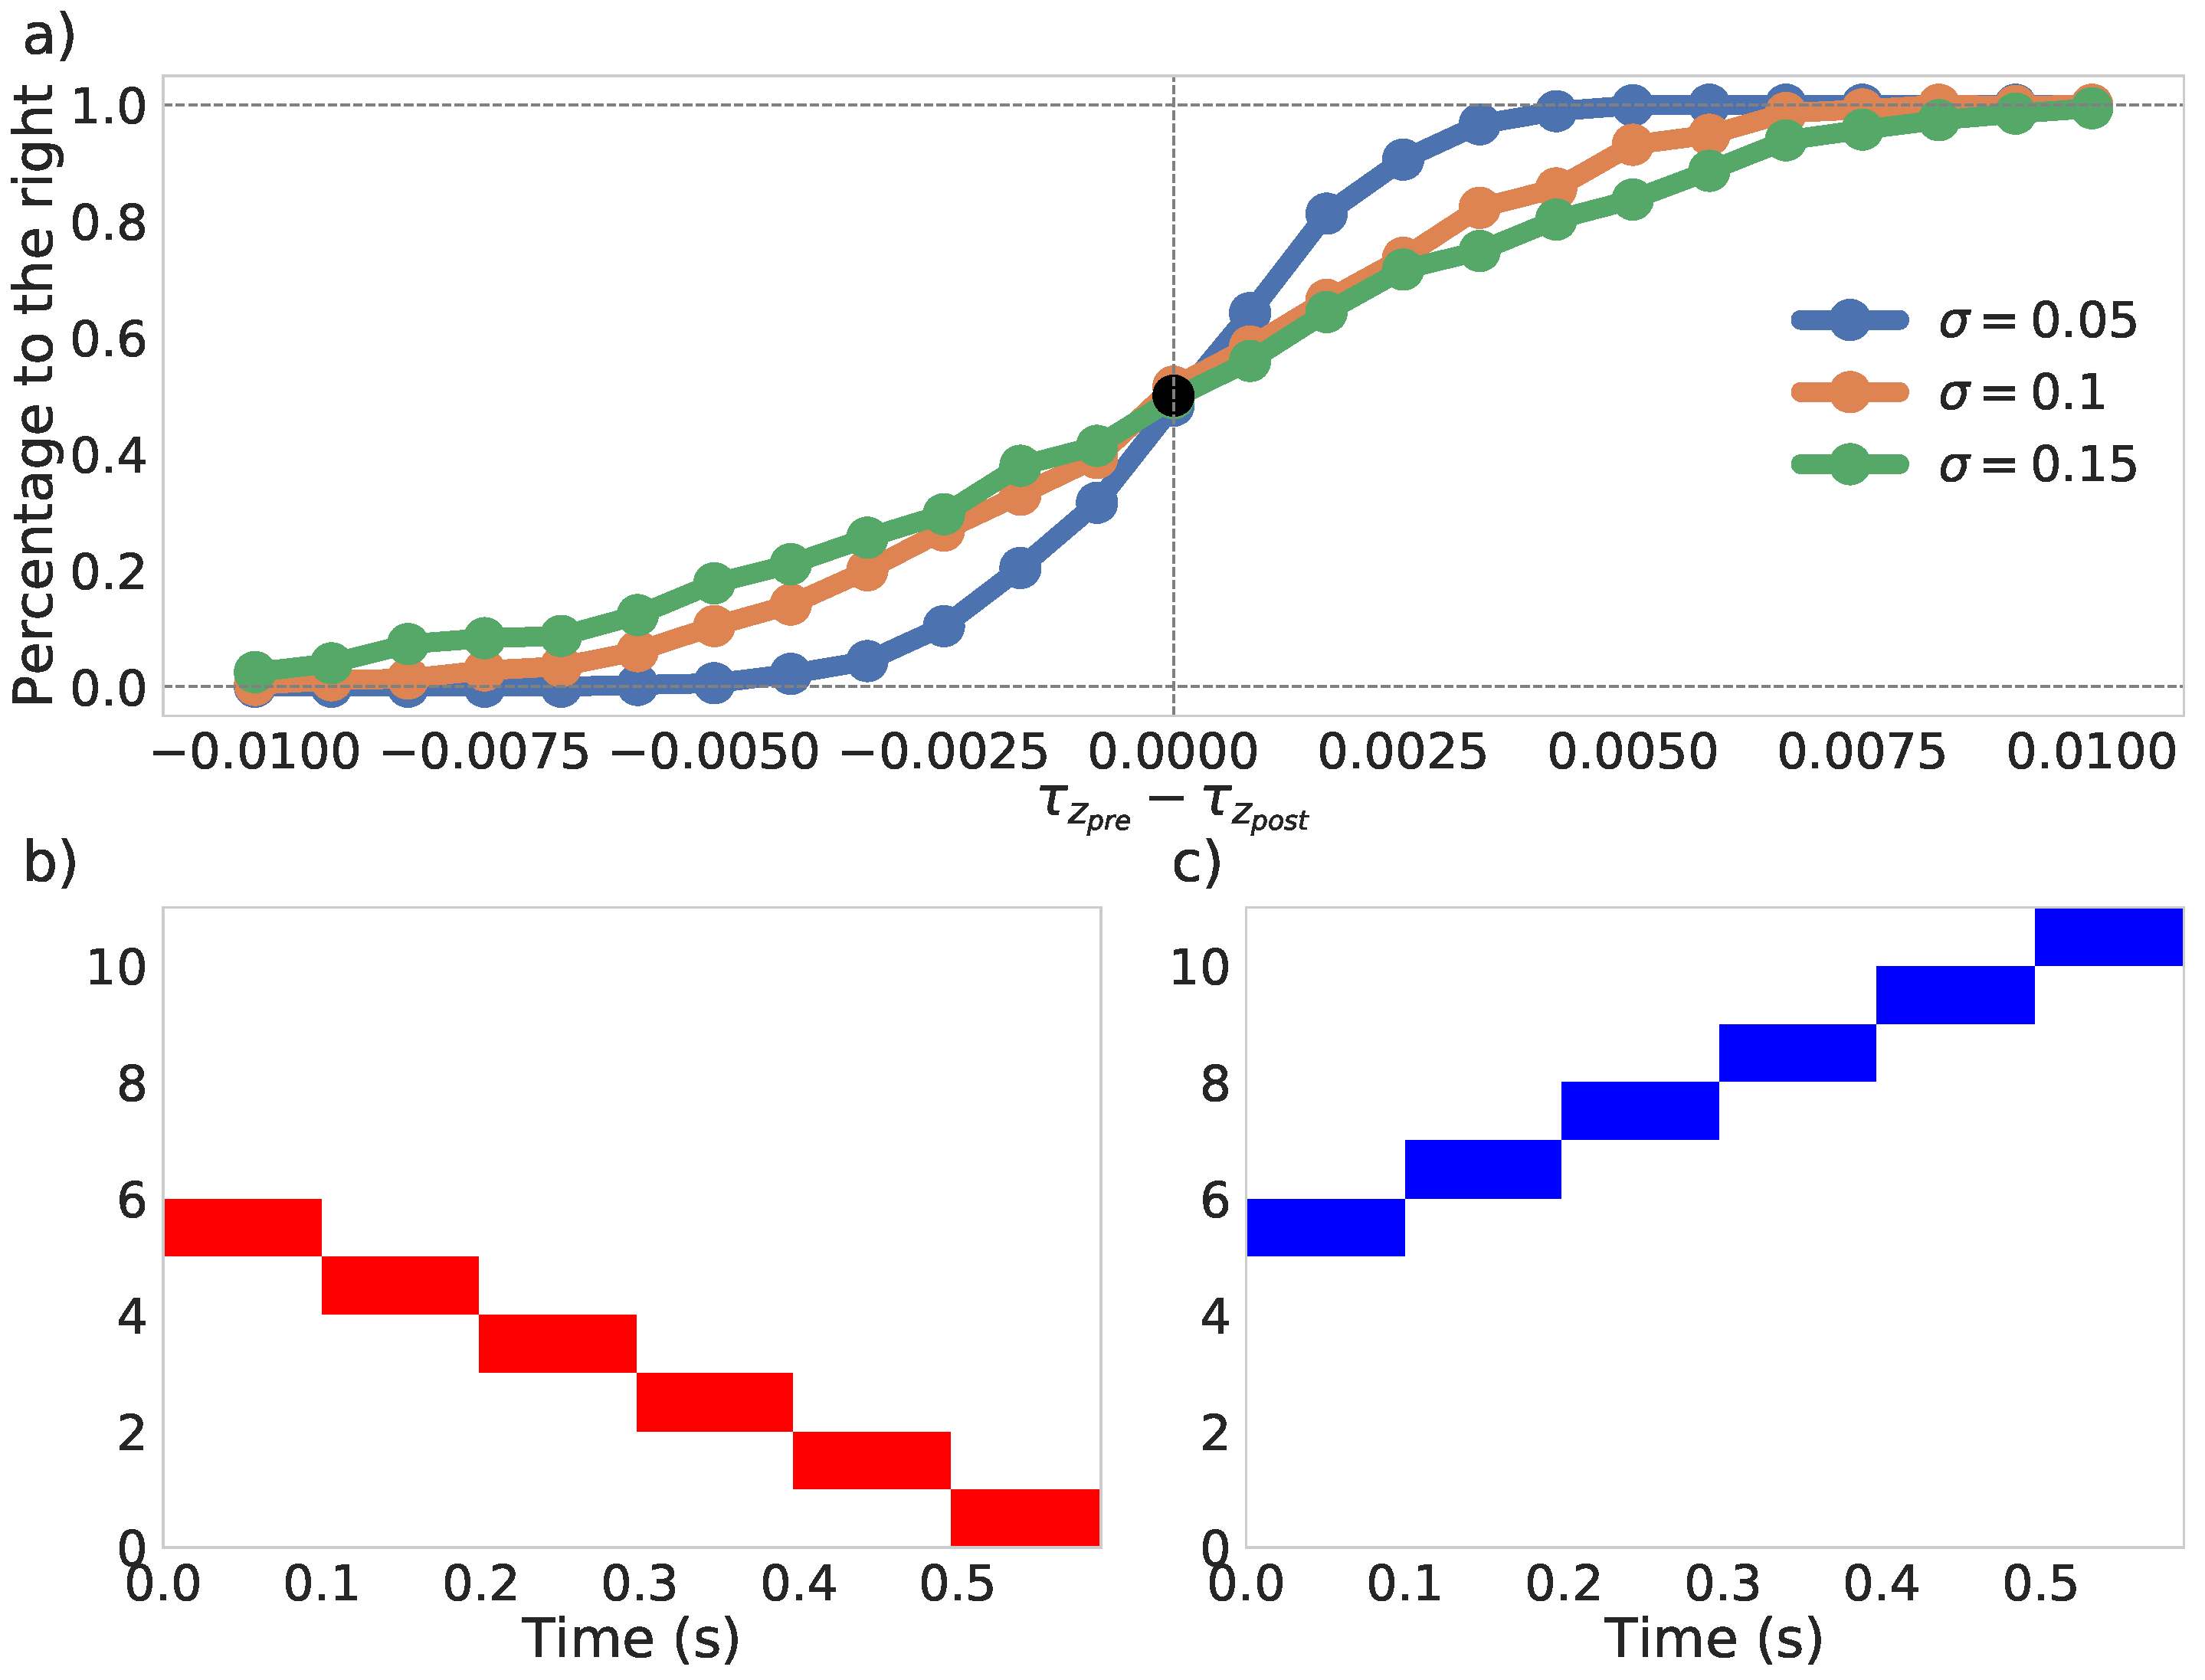
\includegraphics[scale=0.20]{asymmetry.pdf}
\caption{$\tau_z$ effects on sequence recall direction. }
\label{fig:z-assymetry}
\end{figure}

\subsection{Time encoding}
\begin{figure}[H]
\centering
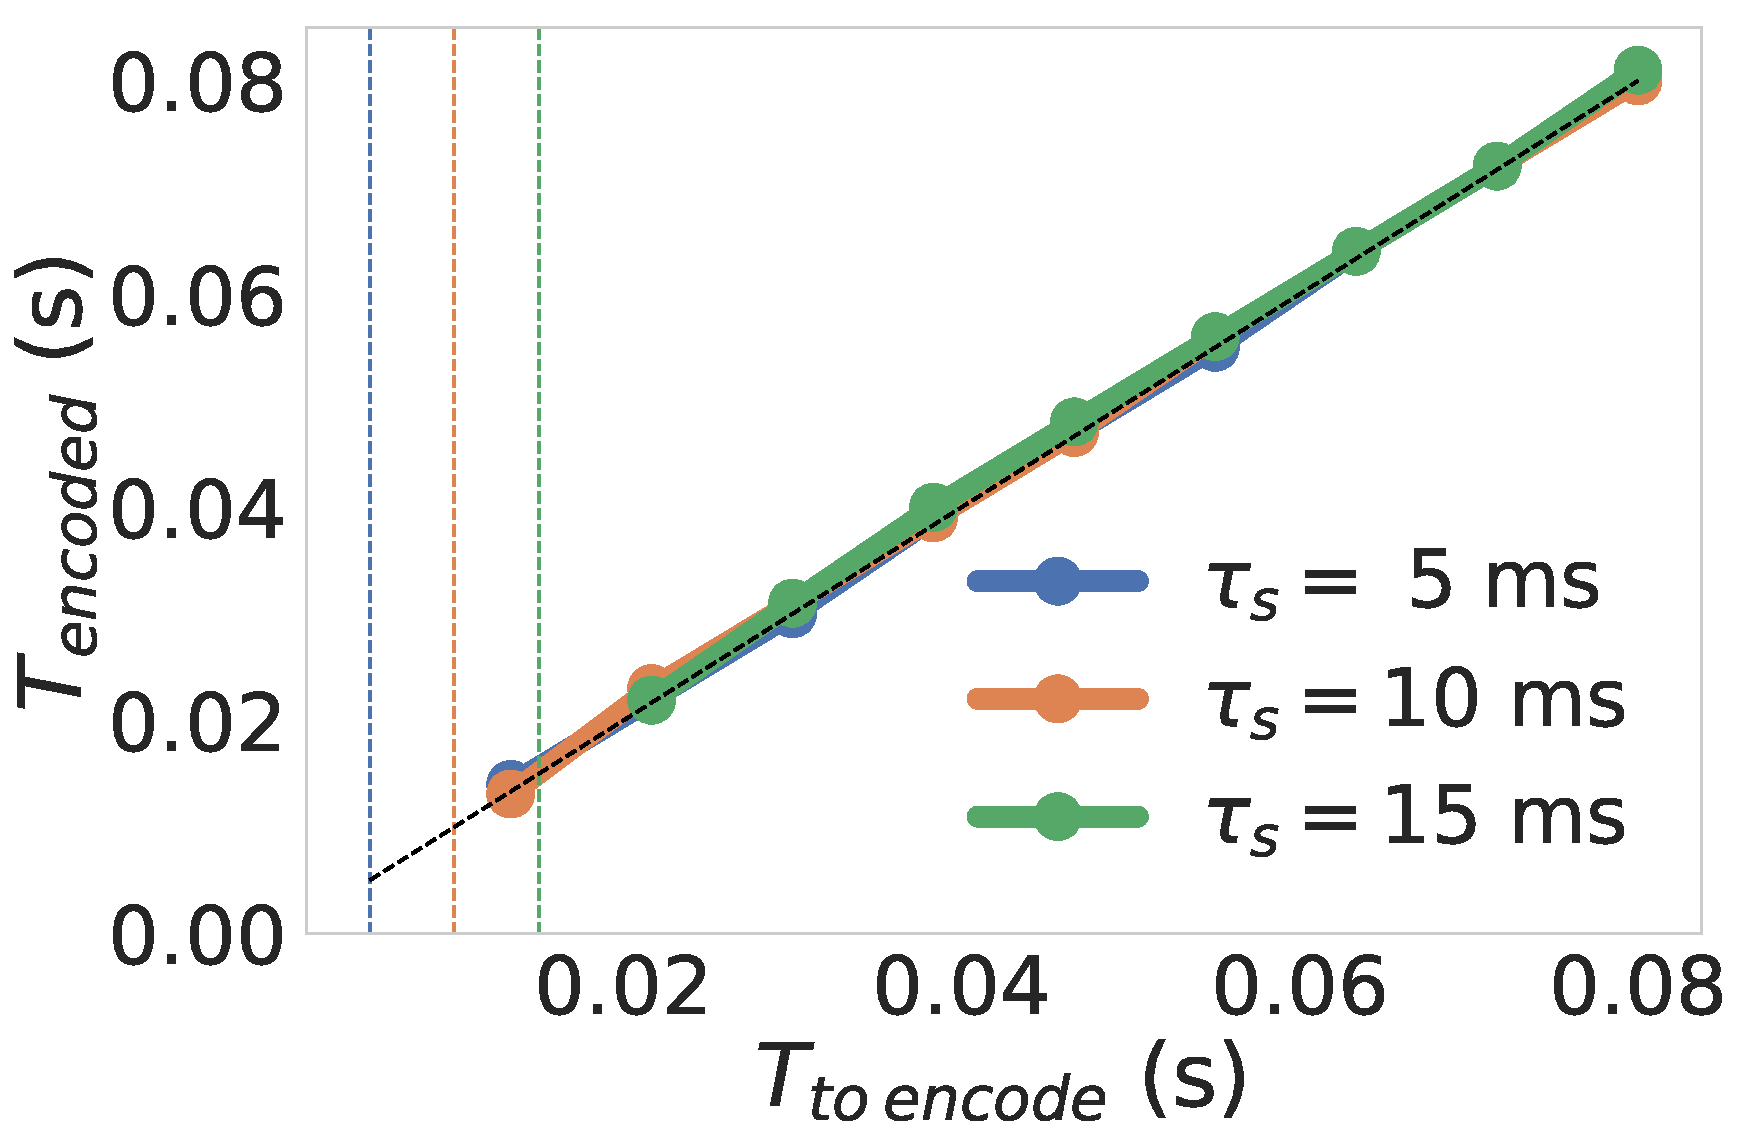
\includegraphics[scale=0.40]{time_encoding.pdf}
\caption{Minimal time encoding. In the x axis we have a particular time that we wish we encode as the persistent time of an attractor. In the y axis we have the time that is actually encoded through the method of fixing the adaptation gain. The leftmost points indicate the minimal possible encoding and after that the time was not encoded successfully. Vertical dashed lines represent the value of $\tau_s$ used for the simulation. We chose the value the middle value of $\tau_s=10 \: ms$  as our $T_{wining}$ (the minimal amount of activation necessary to appear on the sequence).}
\label{fig:min_time_encoding}
\end{figure}

\subsection{Sensitivity calibration}

\begin{figure}[H]
\centering
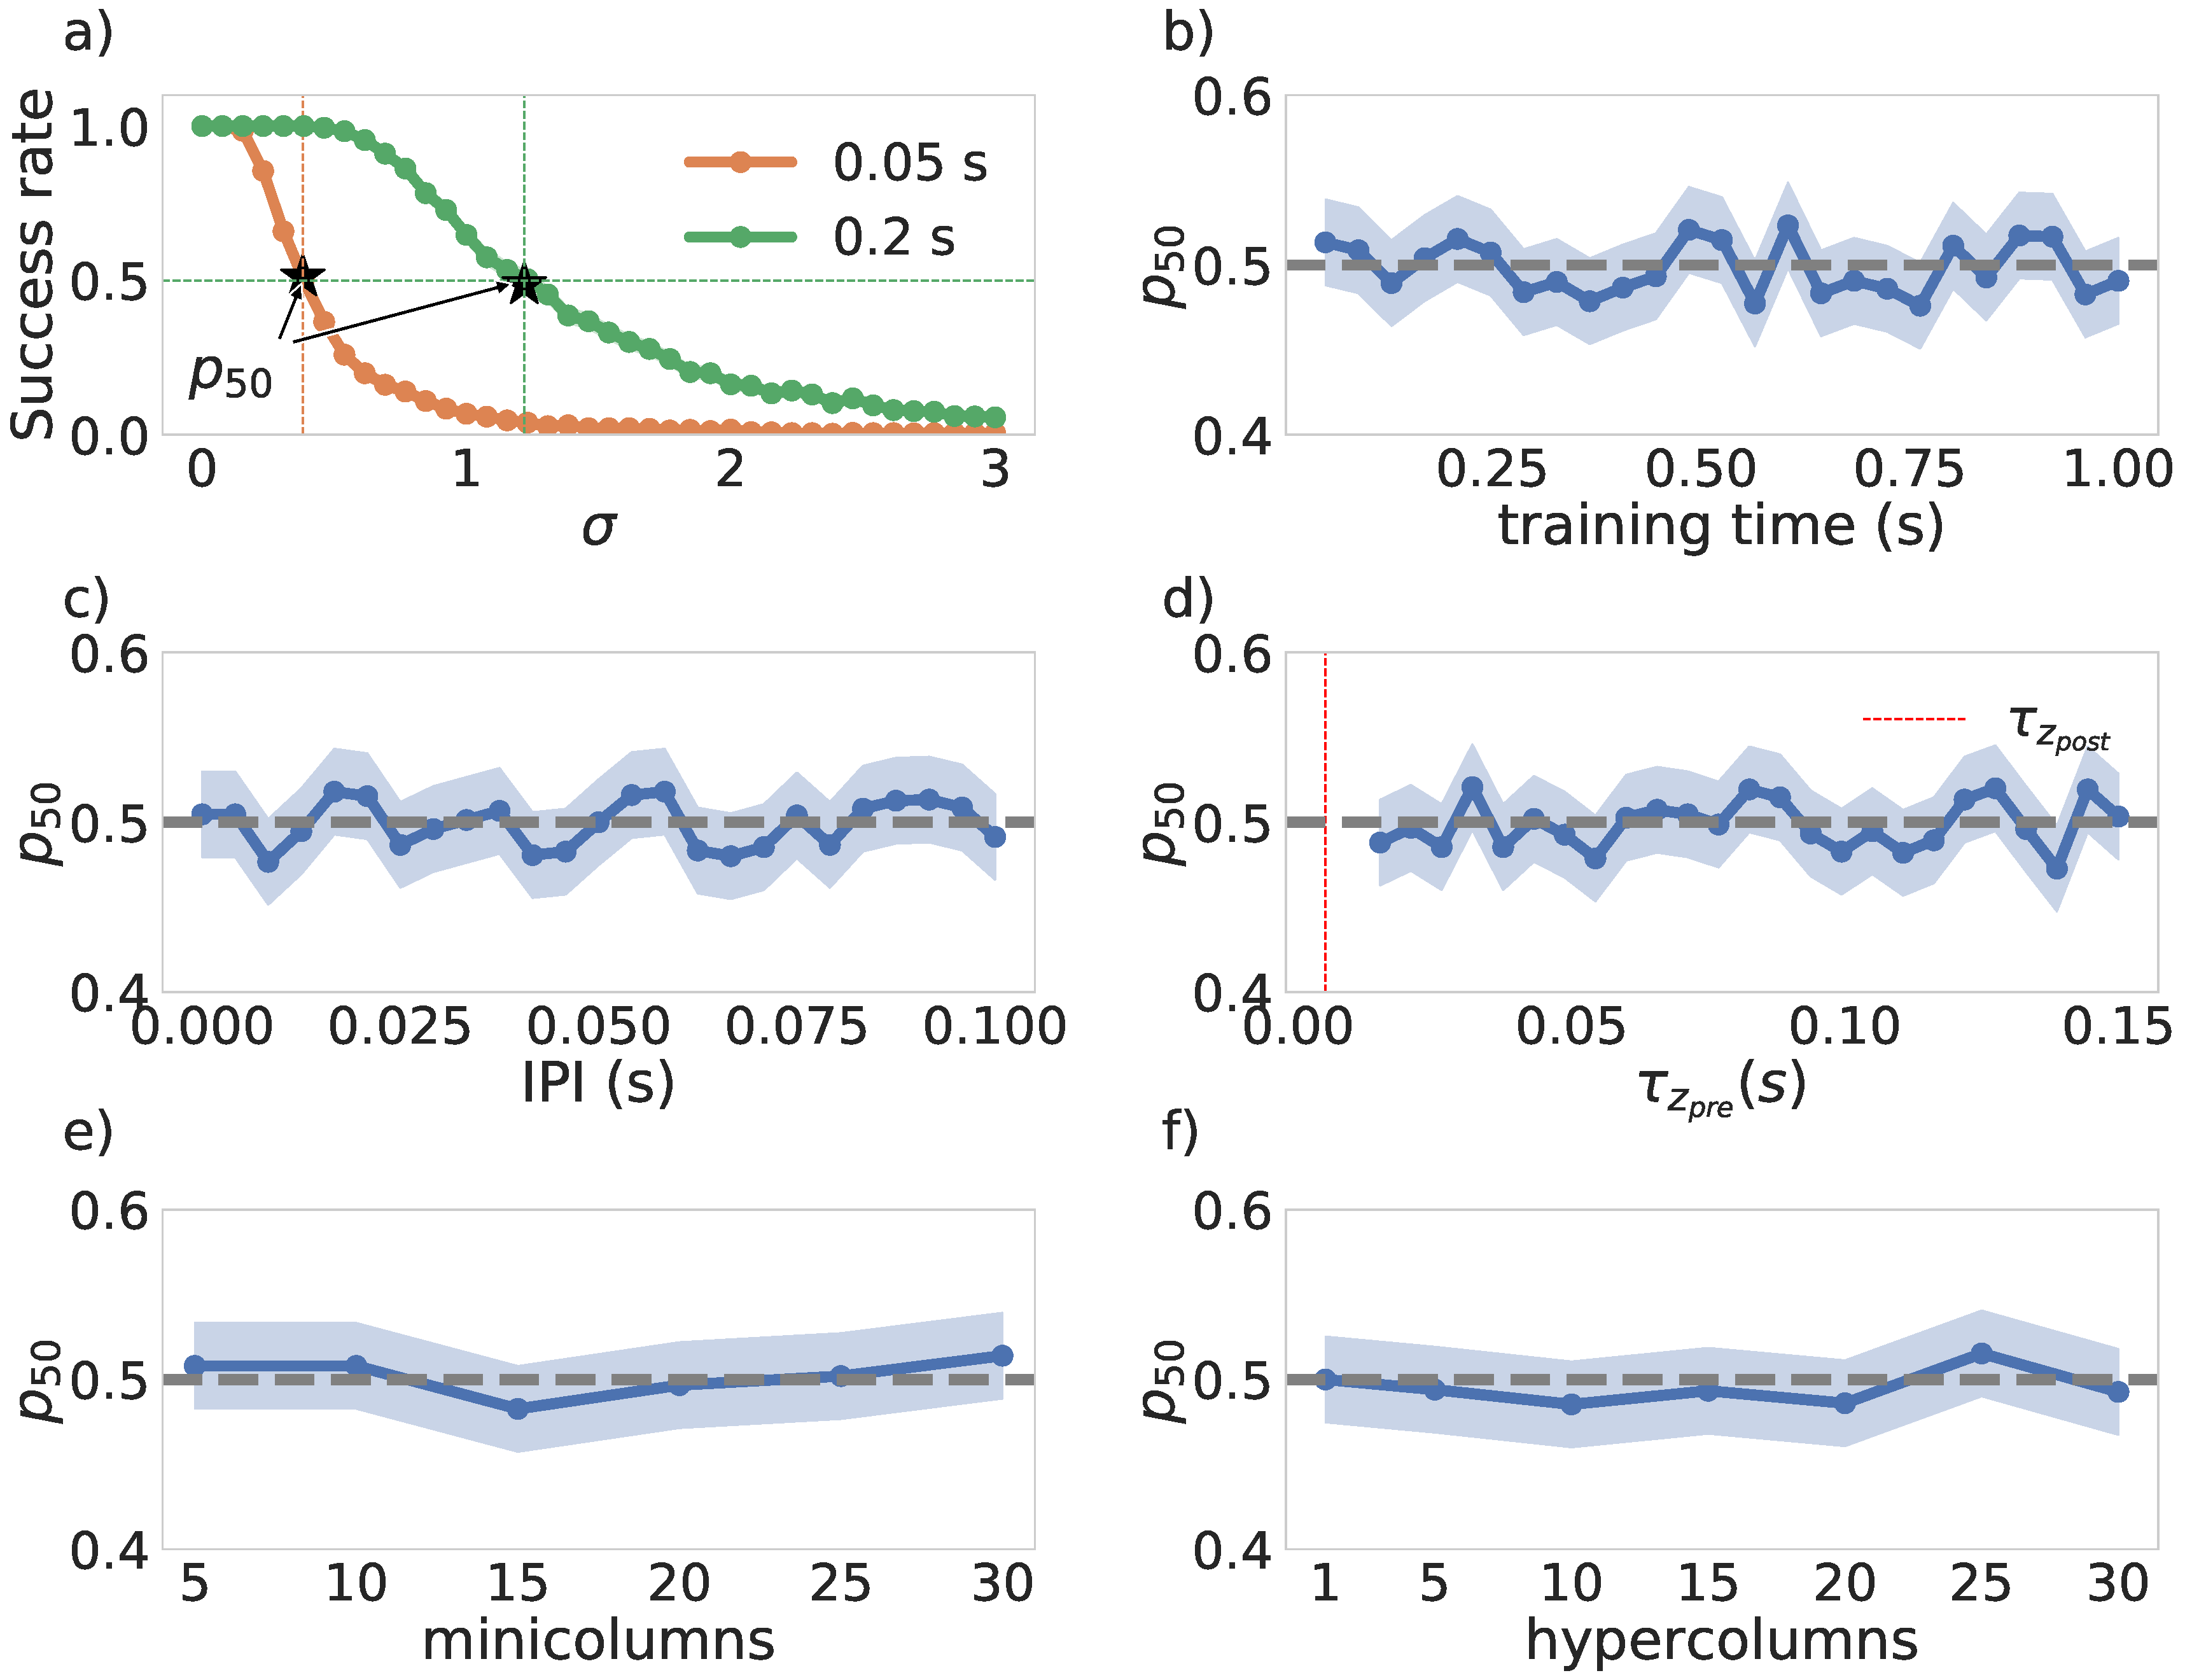
\includegraphics[scale=0.20]{noise_estimates.pdf}
\caption{Calibration of $\sigma_{50}$ estimation.}
\label{fig:noise_calibration}
\end{figure}

\begin{figure}[H]
\centering
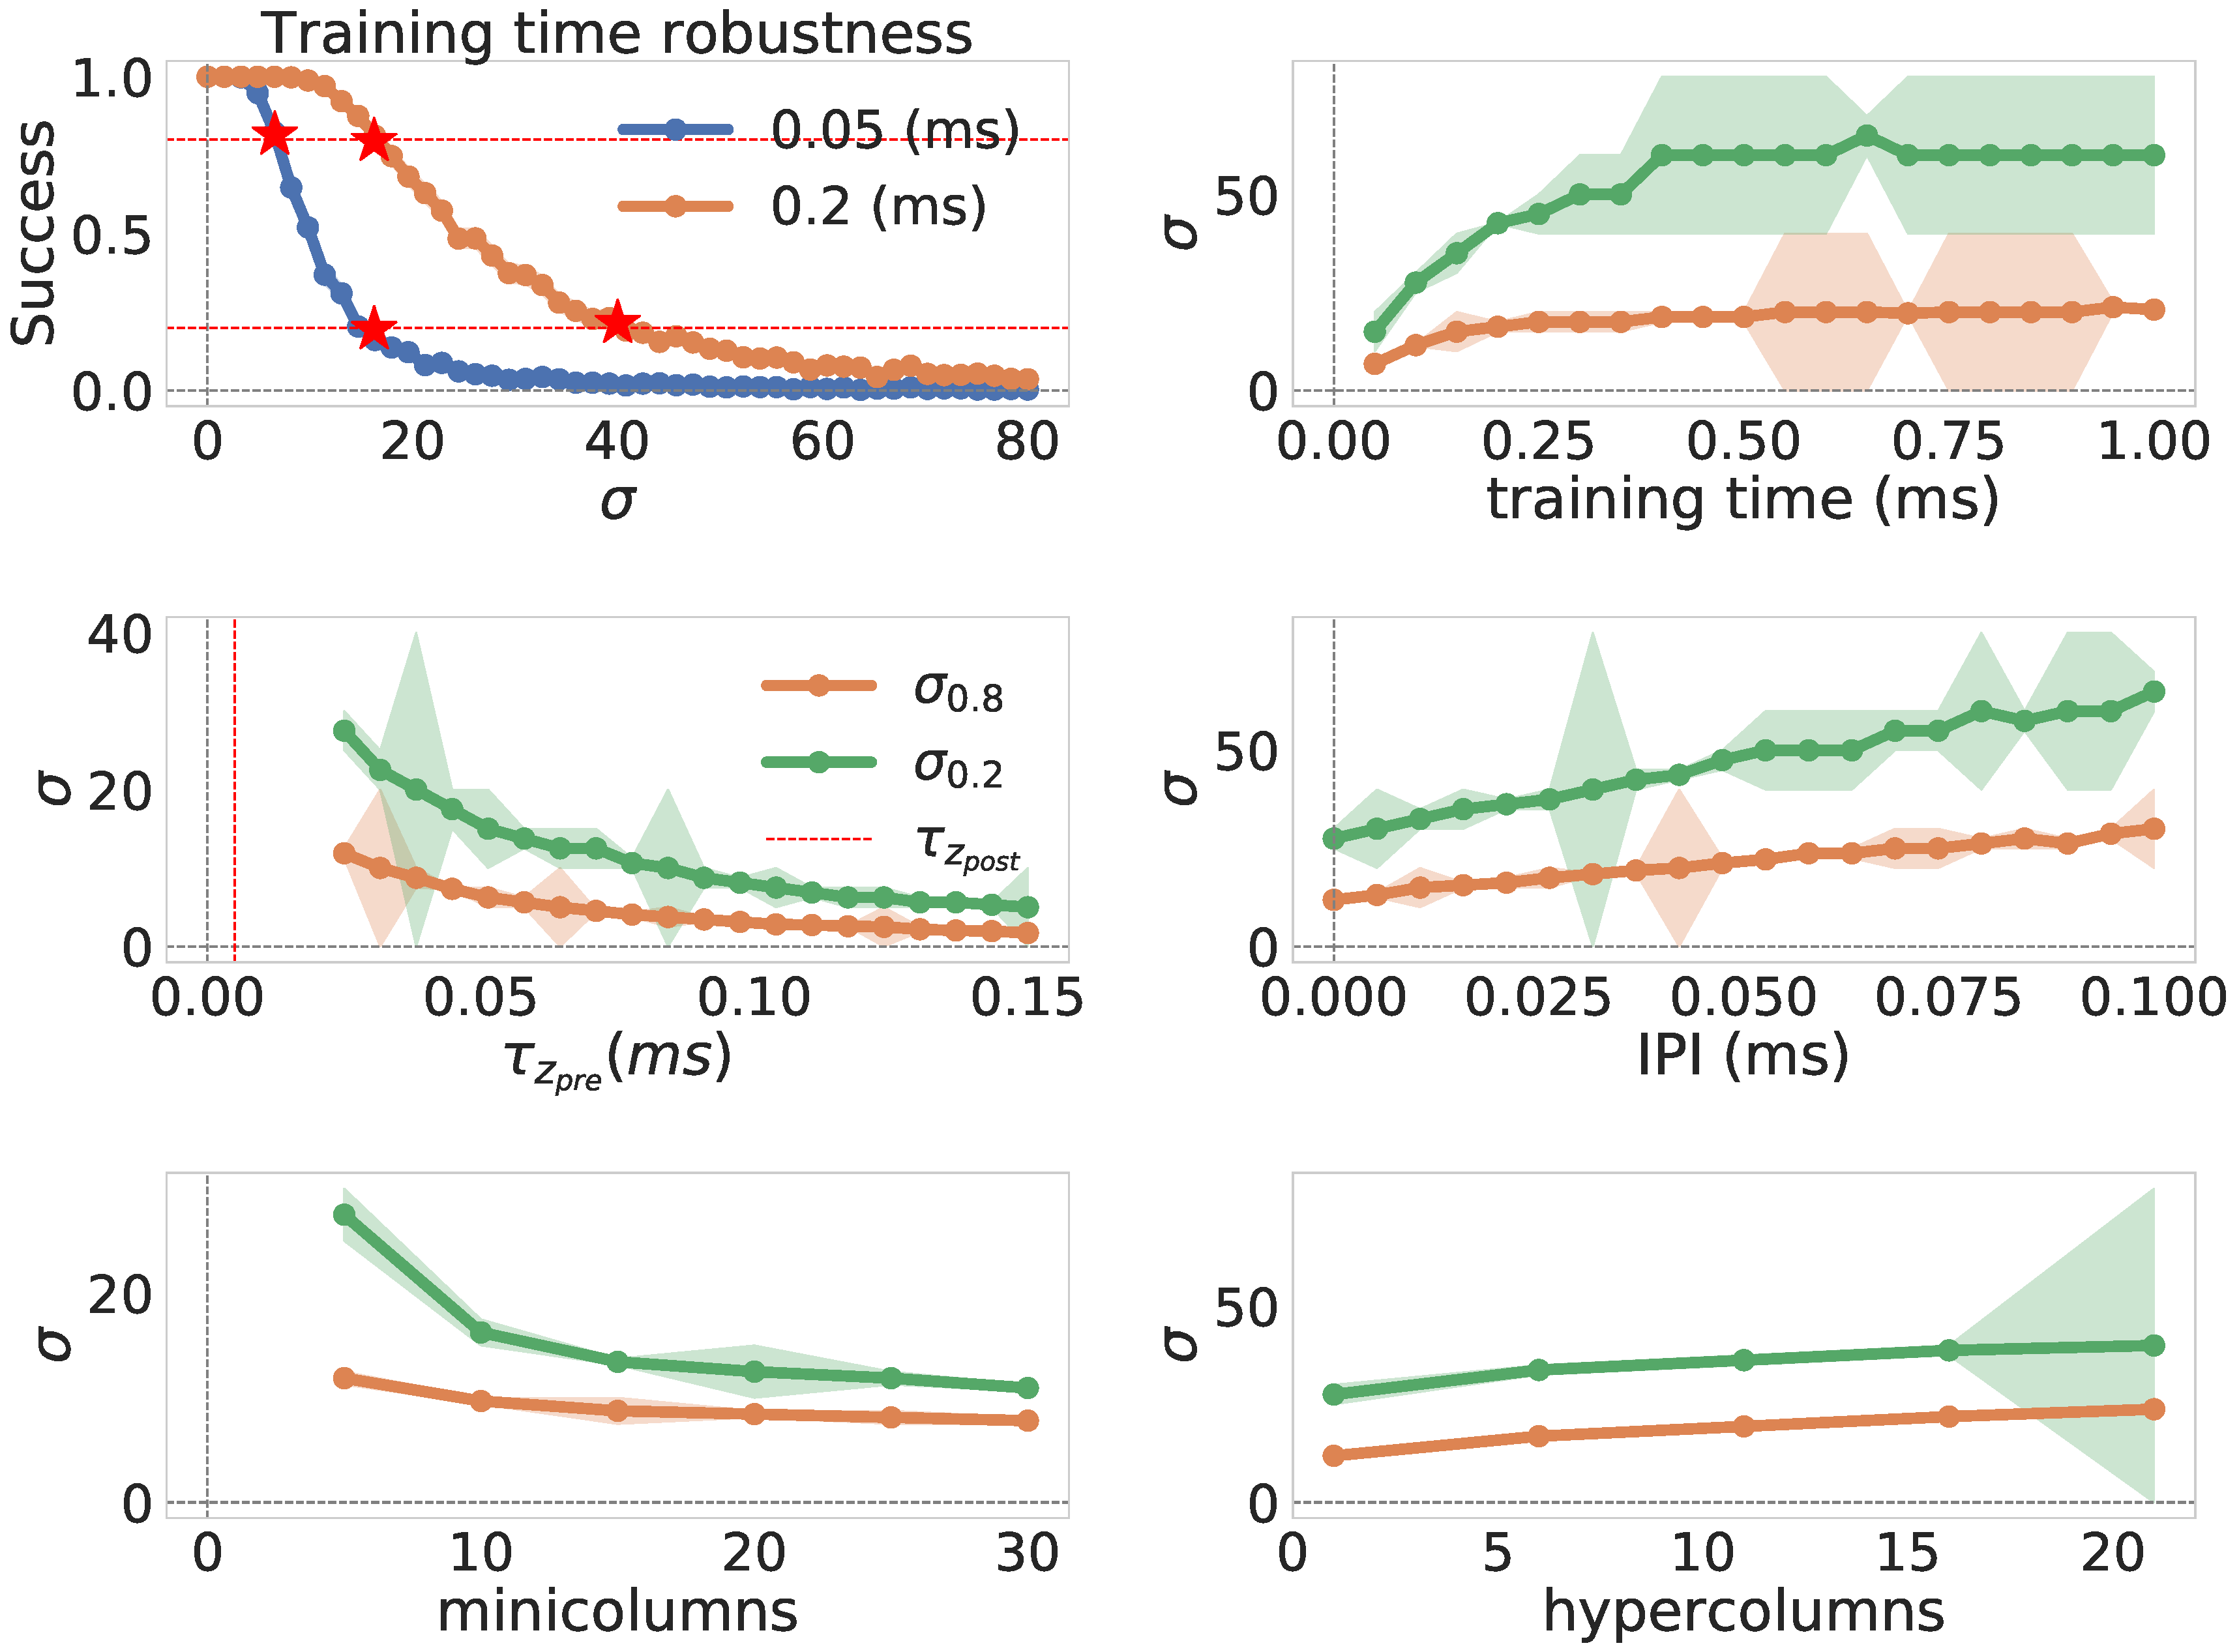
\includegraphics[scale=0.20]{noise_robustness_appendix.pdf}
\caption{$\sigma_{80}$ and $\sigma_{20}$ characterization}
\label{fig:appendix_noise_sensitivity}
\end{figure}


\bibliographystyle{unsrt}
\bibliography{references.bib}

\end{document}